\chapter{\label{ch:proj1_GLR}On the Impact of Sample Size in Reconstructing Noisy Graph Signals: Graph Laplacian Regularised Reconstruction}

\section{Introduction}




\begin{table}[h]
\caption{Structure of Theoretical Results}
\centering
\begin{tabular}{@{} l   c c @{}}
\toprule
 & \multicolumn{2}{c}{GLR} \\
\cmidrule(lr){2-3}
{} & Full-band Noise & Bandlimited Noise \\
\midrule
\emph{Simplification}  & {$\set{N}$ vs $\set{S}$}   & {$\set{N}$ vs $\set{S}$}  \\
\midrule
\emph{Characterisation} & {Corr \ref{corr:main_GLR_iff}} & {Corr \ref{corr:main_GLR_iff}} \\
\midrule
\emph{Existence} & Thm \ref{thm:main_GLR_exist} & Thm \ref{thm:main_GLR_bl}  \\
\midrule
\emph{Asymptotics} &  Propn \ref{propn:GLR_big_N} & Propn \ref{propn:GLR_big_N_bl}\\
\bottomrule
\end{tabular}
\label{tbl:general_theory}
\end{table}

\section{Theoretical Results}
\subsection{GLR with full-band noise}
\label{sec:GLR_full_band}
In this subsection, we show how decreasing sample size can decrease MSE under GLR reconstruction and full-band noise. 


\subsubsection{\bs{Overview and Simplification}}
We start by trying to simplify Theorem \ref{main_general}. Table \ref{tbl:GLR_Reconstruction_Delta} contains no $\times$ scenarios and so the `single vertex' simplification cannot eliminate any conditions in Theorem \ref{main_general}: surprisingly, $\matr{R}_{\set{S} \backslash \{ v \}}$ can be \emph{less} biased than $\matr{R}_{\set{S}}$ for GLR, which can be observed experimentally.
Instead, as we focus on tractability and showing that it is possible to reduce sample size to reduce MSE, rather than fully characterizing all such cases, we pick a situation where $\Delta_{1} \geq 0$ so we can simplify Theorem \ref{main_general}. Specifically, we compare the full observation set $\set{S}=\set{N}$ to a subset of it, which we call the `full observation' simplification. As it is hard to interpret what reconstruction means under full observation \cite{chen2017GLRbias}, our results should be understood as approximately showing that reducing the sample size from nearly full observation to some smaller size may reduce MSE.

Our approach is then as follows. We first characterise under exactly which conditions a sample set $\set{S} \subset \set{N}$ is better than $\set{N}$ (Corollary \ref{corr:main_GLR_iff}). We then show that these conditions must occur if certain graph invariants hold (Theorem \ref{thm:main_GLR_exist}). Finally, we analyse the parameters in Theorem \ref{thm:main_GLR_exist} to obtain a `suggested sample size' (Remark \ref{remark:mopt}) and show the conditions still occur as $N \to \infty$ (Proposition \ref{propn:GLR_big_N}). 

\subsubsection{\bs{Characterisation}}
We first present the following Corollary of Theorem \ref{main_general}.

\begin{corollary}
    \label{corr:main_GLR_iff}
    Assume GLR and that $k > 1$. Consider a non-empty sample set $\set{S} \subset \set{N}$.  Then 
    \begin{equation}
        \tau(\set{N},\set{S}^{c}) = \frac{k}{N} \cdot \frac{\Delta_{2}(\set{N},\set{S}^{c})}{-\Delta_{1}(\set{N},\set{S}^{c})} \label{eq:main_GLR_simplified_tau}
    \end{equation}
    and $\set{S}$ is better than $\set{N}$ if and only if one of the following conditions is met:
        \begin{subnumcases}{ \label{eq:GLR_corol_iff_overall} }
        \text{SNR} < \tau(\set{N}, \set{S}^{c}) &and $ \msubgen[\set{S}^{c},\{2,\ldots,k\}]{\matr{U}} \neq \matr{0}$ \label{eq:GLR_corol_iff}\\
        0 < \Delta_2(\set{N},\set{S}^{c}) &and $ \msubgen[\set{S}^{c},\{2,\ldots,k\}]{\matr{U}} = \matr{0}$. \label{eq:GLR_corol_iff_weird}
\end{subnumcases}
where $\msubgen[\set{S}^{c}, \{2,\ldots,k\}]{\matr{U}} = \vect{0}$ corresponds to any $k$-bandlimited signal always being constant on all of $\set{S}^{c}$.
\end{corollary}
\begin{proof}[Proof Sketch]
    We use Cauchy-Schwartz and Lemma \ref{lemma:GLR_full_observation_MSE} to lower bound $\xi_{1}(\set{S})$ and show that either all $k$ columns of $\matrsubU{N}$ are eigenvectors of $\proj{S} + \mu\matr{L}$ (which is exactly when $\msubgen[\set{S}^{c},\{2,\ldots,k\}]{\matr{U}} = \matr{0}$) and $\Delta_{1}(\set{N},\set{S}^{c}) = 0$, corresponding to (\ref{eq:GLR_corol_iff_weird}), or $\Delta_{1}(\set{N},\set{S}^{c}) < 0$, corresponding to (\ref{eq:GLR_corol_iff}). We then apply Theorem \ref{main_general}. See Appendix \ref{app:proof_main_GLR_iff} for a full proof.
\end{proof}


We now explain the conditions in Corollary \ref{corr:main_GLR_iff}. Condition (\ref{eq:GLR_corol_iff}) corresponds to the single case we see in Corollary \ref{main_ls}. Condition (\ref{eq:GLR_corol_iff_weird}) is more of an edge case,  e.g., if $\lambda_{k} < N$ and every vertex in $\set{S}^{c}$ has degree $N-1$ \cite[Corollary 2.3]{merris1998laplacian}. In (\ref{eq:GLR_corol_iff_weird}), $\msubgen[\set{S}^{c}, \{2,\ldots,k\}]{\matr{U}} = \vect{0}$ means any $k$-bandlimited signal will be constant on all of $\set{S}^{c}$. Our proof shows that in the noiseless case this implies that observing $\set{S}^{c}$ will not improve the MSE, i.e., $\text{MSE}_{\set{S} \cup \set{T}_{c}} = \text{MSE}_{\set{S}}$ for any $\set{T}_{c} \subseteq \set{S}^{c}$. %which means that no information can be gained by observing $\set{S}^{c}$ for a $k$-bandlimited signal apart from the component of the signal which is constant (which corresponds to the lowest graph frequency). For GLR reconstruction in the noiseless case, this knowledge does not aid reconstruction as GLR can always perfectly reconstruct constant signals, and unlike LS it cannot use this knowledge to improve reconstruction of the other components of the bandlimited signal. Therefore, if $\msubgen[\set{S}^{c},\{2,\ldots,k\}]{\matr{U}} = \matr{0}$, observing $\set{S}^{c}$ does not improve the expected MSE under GLR reconstruction in the noiseless case (see Appendix \ref{subapp:GLR_iff_proof:idempotent} for a symbolic proof of this statement). 
The other condition in (\ref{eq:GLR_corol_iff_weird}), i.e., $0 < \Delta_2(\set{N},\set{S}^{c})$, corresponds to an increase in sensitivity to noise from reconstructing from those additional vertices. Therefore, condition (\ref{eq:GLR_corol_iff_weird}) says that if $\set{S}^{c}$ reveals nothing new about the underlying signal and also makes the reconstruction more sensitive to noise, one should not observe $\set{S}^{c}$ and only observe $\set{S}$.


%Instead of exactly characterising the behaviour on removing a single vertex from an arbitrary sample set $\set{S}$, we proceed with our `bound' proof strategy. We consider removing multiple vertices from the full observation set $\set{N}$. We use Theorem \ref{main_general} by bounding $\tau(\set{N},\set{S}^{c})$. We do so by bounding $\xi_{i}(\set{S})$ and $\xi_{i}(\set{N})$, and thence bounding $\Delta_{i}(\set{N}, \set{S}^{c})$. This gives a characterisation of when removing all but a sample set $\set{S}$ improves $\set{N}$. We call this bound $\tau_{lb}$.

\subsubsection{\bs{Existence}}
Like Corollary \ref{main_ls}, Corollary $\ref{corr:main_GLR_iff}$ does not show that any set $\set{S}$ is ever better than $\set{N}$, i.e., that $\tau(\set{N},\set{S}^{c}) > 0$ ever happens. {\color{black} As described in Section \ref{sec:every_x}, we will find $\set{S}$ s.t. $\Delta_{2}(\set{N},\set{S}^{c}) > 0$. We illustrate our proof method in Fig.~\ref{fig:GLR_diagram}.

\begin{figure}[t]
    \centering
    %\resizebox{\width}{0.75\columnwidth}
    \resizebox{0.75\width}{0.75\height}
    {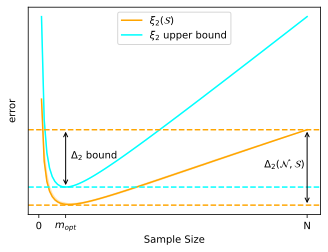
\includegraphics[width=\columnwidth]{figures/proj1/plots/GLR_diagram/diagram_GLR.png}}
    \caption{Proof direction to show $\Delta_{2}(\set{N},\set{S}^{c}) > 0$}
    \label{fig:GLR_diagram}
\end{figure}

\noindent Fundamentally, our approach rests on the fact that $\xi_{2}$, which is approximately proportional to $\text{MSE}_{\set{S}}$ at high noise levels, is  approximately U-shaped, and we can use an upper bound to approximate the minimum and thus bound $\Delta_{2}(\set{N},\set{S}^{c})$ below. Explicitly, our method to show $\Delta_{2}(\set{N},\set{S}^{c}) > 0$ is:
\begin{enumerate}
    \item Find an upper bound $B(\cdot)$ for $\xi_{2}(\set{S})$ that only depends on $\matr{L}$ and $|\set{S}|$, not on $\mu$ or the choice of $\set{S}$.
    \item Find the sample size $m_{opt}$ that minimises the bound and show $m_{opt} < N$.
    \item Identify when $\xi_{2}(\set{N}) - B(m_{opt}) > 0$ (this is the `$\Delta_{2}$ bound' in Fig. \ref{fig:GLR_diagram}). As this quantity is a lower bound for $\Delta_{2}(\set{N},\set{S}^{c})$ this shows that $\Delta_{2}(\set{N},\set{S}^{c})>0$ for any $\set{S}$ of size $m_{opt}$.
    \item Bound $\Delta_{1}$ using the same tools and use these to lower bound $\tau(\set{N}, \set{S}^{c})$
\end{enumerate}
We see that $m_{opt}$ suggests an `optimal sample size', in the sense that the $\xi_{2}$ upper bound approximates $\xi_{2}$, and we can optimise it as a surrogate. Following step 1, we now bound $\xi_{2}(\set{S})$.

\iffalse
To show that $\tau$ can be positive under GLR, we bound it from below similarly to Theorem \ref{thm:noiseless_optimality_means_noise_sensitivity}.{\color{black} We start with a weaker, easier-to-understand version of the full theorem:
\fi

\begin{lemma}
\label{lemma:GLR_xi_2_bound_main}
    Let $\lambda_{i}$ be the eigenvalues of $\matr{L}$, the combinatorial Laplacian. Let $|\set{S}| = m$. Then
    \begin{align}
        \xi_{2}(\set{S}) &\leq r\frac{N}{m} + \sum_{i=2}^{m} \omega\left(\max\left[1,\frac{\lambda_{N+2-i}}{\lambda_{i}}\right]\right)  \label{eq:xi_2_GLR_bound_strong}
        \\ 
        &\leq r\frac{N}{m} + r(m -1) . \label{eq:xi_2_GLR_bound_weak}
    \end{align}
    where we define $B(m)$ to be the RHS of (\ref{eq:xi_2_GLR_bound_strong}) and where
    \begin{align}
        \omega(x) &= \frac{1}{4}\left(\sqrt{x}+ \frac{1}{\sqrt{x}} \right)^{2}, \quad
        r = \omega\left(\frac{\lambda_{N}}{\lambda_{2}}\right)
    \end{align}
   and the summation in (\ref{eq:xi_2_GLR_bound_strong}) is 0 if $m = 0$ or $1$. 
    
\end{lemma}
\begin{proof}
    Decompose $\matr{R}_{\set{S}}$ and apply Kantorovich's inequality. See Appendix \ref{app:proof_unif_ub_xi_2}.
\end{proof}

The function $\omega$ arises from the Kantorovich inequality, commonly used in variance bounds \cite{khatri1982some, householder1965kantorovich}. $\omega$ is an increasing function and for $x>1, \omega(x) \leq x$; this means $r$ increases with $\frac{\lambda_{N}}{\lambda_{2}}$. We discuss $r$ in more detail in Appendix \ref{app:GLR_sensitivity}.

As mentioned, in step 4 we need a bound on $\xi_{1}(\set{S})$ to lower bound $\tau(\set{N},\set{S}^{c})$. The shape and accuracy of this bound do not affect the core of our argument, only how tight our approximation of $\tau$ is. Therefore, we leave it in Appendix \ref{app:proof_unif_ub_xi_1_MSE}; the term $B_{k}(m)$ it introduces in the proof is a tightening of $B(m)$ ($B_{k}(m) < B(m)$) and is explained in Appendix  \ref{app:GLR_bandlimited}.

Following steps 2, 3 and 4 using the bound $B(m)$ in Lemma \ref{lemma:GLR_xi_2_bound_main} yields: 

\begin{theorem}
\label{thm:main_GLR_exist}
{\color{black} Let $B(m)$ be defined as in Lemma \ref{lemma:GLR_xi_2_bound_main} and let $m_{opt}$ be the sample size minimising $B$.
    \begin{flalign}
        &\text{If} \hspace{0.35\columnwidth} B(m_{opt}) < N& \label{eq:GLR_exist_thm_B_constraint}
    \end{flalign}
then $m_{opt} < \lceil\frac{N+1}{2}\rceil$. Furthermore, $\exists \mu_{ub} > 0$ and $\tau_{GLR}(\mu) > 0$ s.t. under GLR with parameter $\mu \in (0, \mu_{ub})$,
\begin{flalign}
        &\text{if} \hspace{0.3\columnwidth} \textrm{SNR} < \tau_{GLR}(\mu)&
    \end{flalign}

    \noindent then,  \emph{any} sample set $\set{S}$ of size $m_{opt}$ is better than $\set{N}$.}
\end{theorem}
\begin{proof}[Proof Sketch] 
We prove that for any $\mu$, $\xi_{1}(\set{S}) \leq k + B_{k}(m)$ and $\xi_{2}(\set{S}) \leq B(m)$ via Lemmas \ref{lemma:GLR_xi_2_bound_main} and \ref{lemma:GLR_xi_2_bound_main_bl}. We also show $\xi_{1}(\set{N}) = \sum_{i=1}^{k} \left(1 - \frac{1}{1+\mu\lambda_{i}}\right)^{2}$ and $\xi_{2}(\set{N}) = \sum_{i=1}^{N} \left({1+\mu\lambda_{i}}\right)^{-2}$.
We use these to bound $\Delta_{i}$, and finally apply Corollary \ref{corr:main_GLR_iff} as our conditions mean $\Delta_{2}(\set{N},\set{S}^{c}) > 0$.  See Appendix \ref{app:Proof_thm_main_GLR_exist} for a full proof.
\end{proof}
}
 We contrast Theorems \ref{thm:noiseless_optimality_means_noise_sensitivity} and \ref{thm:main_GLR_exist}. Theorem \ref{thm:noiseless_optimality_means_noise_sensitivity} provides necessary and sufficient conditions. Theorem  \ref{thm:main_GLR_exist}, while still useful, only provides sufficient conditions. 
 Theorem \ref{thm:noiseless_optimality_means_noise_sensitivity} applies to any graph, but only to sample sets chosen under noiseless-optimal sampling schemes, while Theorem \ref{thm:main_GLR_exist} has no requirement on sampling schemes, but only applies to graphs which fulfill certain graph invariants. % for when a subset is better than a sample set of any size chosen under sequential noiseless-optimal sampling schemes under LS. Theorem \ref{thm:main_GLR_exist} only provides sufficient conditions for when removing samples from the full observation set $\set{N}$ reduces MSE under GLR. In this sense, Theorem \ref{thm:main_GLR_exist} is a weaker (nevertheless still useful) result.
 %Finally, both theorems require no constraints on the set of nodes removed for their results to hold.

{\color{black}
Because of the difficulty in writing down an analytic form for $m_{opt}$, the parameters in Theorem \ref{thm:main_GLR_exist} -- $m_{opt}$, $\mu_{ub}$ and $\tau_{GLR}$ -- are difficult to analyse. To better understand  we present a version of Theorem \ref{thm:main_GLR_exist} instead based on  
the weaker bound (\ref{eq:xi_2_GLR_bound_weak}). This bound is a linear transformation of $\frac{N}{m} + m$ and so is clearly U-shaped and has an minimum at $m=\sqrt{N}$, and thus following steps 2, 3 and 4 yields the following proposition:

\begin{propn}
\label{propn:GLR_simple}
    Let $\bar{\lambda} = \frac{1}{N}\sum_{i=1}^{N}\lambda_{i}$ be the mean eigenvalue of $\matr{L}$ and let $r$ be defined as in Lemma \ref{lemma:GLR_xi_2_bound_main}.  
    \begin{flalign}
        &\text{If} \hspace{0.35\columnwidth} 2r\sqrt{N} < N& \label{eq:weak_GLR_constraint}
    \end{flalign}
    Let
    \begin{align}
        \mu_{ub\_weak} &= \bar{\lambda}^{-1}\left(\sqrt[4]{N}\cdot ({2r})^{-\frac{1}{2}} - 1 \right) \\
        \tau_{GLR\_weak} &=  \frac{\sqrt{N}(1 + \mu\bar{\lambda})^{-2} - 2r}{\sqrt{N} + 2r \cdot \frac{N}{k} }
    \end{align}
    then under GLR with parameter $\mu \in (0,\mu_{ub\_weak})$, if
    \begin{equation}
        \text{SNR} < \tau_{GLR\_weak}(\mu)
    \end{equation}
    then \emph{any} sample set $\set{S}$ of size $\lceil\sqrt{N}\rceil$ is better than $\set{N}$.
\end{propn}
\begin{proof}[Proof Sketch]
    We bound $\xi_{1}(\set{S})$ and $\xi_{2}(\set{S})$ in terms of $r\left(\frac{N}{m} + m - 1\right)$, which is minimised at $m = \sqrt{N}$. We explicitly compute $\xi_{i}(\set{N})$ and apply Corollary \ref{corr:main_GLR_iff}. See Appendix \ref{app:proof_propn_GLR_simple} for a full proof.
\end{proof}


%This proposition provides sufficient conditions for reducing sample size to reduce MSE; unlike Theorem \ref{thm:noiseless_optimality_means_noise_sensitivity}, which provides both necessary and sufficient conditions. 

Proposition \ref{propn:GLR_simple} is sufficient to show that decreasing sample size can decrease MSE on a restricted class of graph models (e.g. Erdős–Rényi graphs). 
Proposition \ref{propn:GLR_simple} involves several parameters: $r$, $2r\sqrt{N}$, $\mu_{ub\_weak}$ and $\tau_{GLR\_weak}$ which can be interpreted as graph properties (see Appendix \ref{app:GLR_sensitivity} for a detailed explanation and sensitivity analysis). 


Intuitively, we expect the equivalent parameters in Proposition \ref{propn:GLR_simple} and Theorem \ref{thm:main_GLR_exist} to behave similarly; for $m_{opt}$ to behave like $\left\lceil \sqrt{N} \right\rceil$, for $B(m_{opt})$ to behave like $2r\sqrt{N}$ and for $\mu_{ub}$ and $\tau_{GLR}$ to behave like their weak counterparts. We can explicitly show that $m_{opt}$ is $\mathcal{O}(\sqrt{N})$:

\begin{remark}
\label{remark:mopt}
If condition (\ref{eq:GLR_exist_thm_B_constraint}) in Theorem \ref{thm:main_GLR_exist} holds
    then $m_{opt} \in \left[\left\lfloor\sqrt{N}\right\rfloor, \left\lceil\sqrt{rN}\right\rceil \right]$ and $m_{opt} \leq \lceil\frac{N+1}{2}\rceil$.
\end{remark}
\begin{proof}
    See Appendix \ref{app:proof_of_remark_GLR_mopt}.
\end{proof}

}


%We now exactly write down the MSE when $|\set{S}| = N$:

\iffalse
\begin{theorem}
\label{thm:main_GLR_exist}
{\color{black}
Let $0 = \lambda_{1} < \lambda_{2} \leq \ldots \leq \lambda_{N}$ be the eigenvalues of $\matr{L}$ and let
\begin{align}
    %r_{i} &= \left(\frac{1}{2}\sqrt{ \frac{\lambda_{N+i-1}}{\lambda_{i+1}}} +
    r_{i} &= \frac{(\lambda_{i+1} + \lambda_{N+1-i})^{2}}{4\lambda_{i+1}\lambda_{N+1-i}}, \quad r = r_{1} = \frac{(\lambda_{2} + \lambda_{N})^{2}}{4\lambda_{2}\lambda_{N}}, \\
 %\frac{(\lambda_{i+1}+\lambda_{N+1-i})^{2}}{4\lambda_{i+1}\lambda_{N+1-i}} \\
    \rho(m) &= \begin{dcases}
        \sum^{m}_{i=1} r_{i} & \textrm{if }2m \leq N \\
        (2m - N) + \rho\left((N-1)-m\right)    & \textrm{otherwise}
    \end{dcases},\\ 
    B(m) &= \frac{rN}{m} + \rho({m-1}) 
\end{align}
}
    For any sample size $ 0 < m  < N$, let
    \begin{align}
        \mu_{ub}(m) &= \frac{N}{\trace{\matr{L}}} \left( \sqrt{\frac{N}{B(m)}}  -1 \right) \\
        \tau_{{bound}}(\mu,m) &= \frac{\frac{1}{N}\sum_{i=1}^{N}\left({1 + \mu \lambda_{i}}\right)^{-2} - \frac{B(m)}{N}}{1 + \frac{B(m)}{k} - \frac{1}{k}\sum_{i=1}^{k}\left( 1 - \frac{1}{1 + \mu \lambda_{i}}\right)^{2} }.
    \end{align}
    {\color{black}
    Under GLR with parameter $\mu$ where $0 <\mu < \mu_{ub}(m)$,
    \begin{flalign}
        &\text{if} \hspace{0.35\columnwidth} B(m) < N& \label{eq:GLR_exist_thm_B_constraint} \\
        &\text{and} \hspace{0.3\columnwidth} \textrm{SNR} < \tau_{lb}(\mu,m)&
    \end{flalign}
    then,  \emph{any} sample set $\set{S}$ of size $m$ is better than $\set{N}$.}
\end{theorem}
\begin{proof}[Proof Sketch] 
We prove that  for any $\mu$, $\xi_{1}(\set{S}) \leq k + B(m)$ and $\xi_{2}(\set{S}) \leq B(m)$. We also show $\xi_{1}(\set{N}) = \sum_{i=1}^{k} \left(1 - \frac{1}{1+\mu\lambda_{i}}\right)^{2}$ and $\xi_{2}(\set{N}) = \sum_{i=1}^{N} \left({1+\mu\lambda_{i}}\right)^{-2}$.
We use these to bound $\Delta_{i}$, and finally apply Corollary \ref{corr:main_GLR_iff} as our conditions mean $\Delta_{2}(\set{N},\set{S}^{c}) > 0$. See Appendix \ref{app:Proof_thm_main_GLR_exist} for a full proof.
\end{proof}
\fi


%{\color{black}Finally, we would like to experimentally see what our bound looks like and how it corresponds to MSEs. }
The proof of Theorem \ref{thm:main_GLR_exist} leads to an upper bound of $\text{MSE}_{\set{S}}$. {\color{black} We present this upper bound to link the experiments in Section \ref{sec:experiments} with Fig. \ref{fig:GLR_diagram}, which can be considered to be the case where $\sigma^{2} \to \infty$.
\begin{corollary}
\label{corr:unif_ub_xi_1_MSE}
    Let $B(m)$ be defined as in Lemma \ref{lemma:GLR_xi_2_bound_main} and $B_{k}(m)$ be defined as it will be in Lemma \ref{lemma:GLR_xi_2_bound_main_bl}. 
    
    For a sample set $\set{S}$ of size $m$,
    \begin{align}
    \textrm{MSE}_{\set{S}} &\leq (k + B_{k}(m)) + \sigma^{2} \cdot B(m). \label{eq:unif_ub_MSE}
    \end{align}
\end{corollary}
\begin{proof}
By Lemma \ref{lemma:GLR_xi_2_bound_main} \iffalse in Appendix \ref{app:proof_unif_ub_xi_2},\fi $\xi_{2}(\set{S}) \leq B(m)$. By Lemma \ref{lemma:unif_ub_xi_1_GLR} in Appendix \ref{app:proof_unif_ub_xi_1_MSE}, $\xi_{1}(\set{S}) \leq k + B_{k}(m)$. Combining these using (\ref{eq:xi_decomp}) gives the bound.
\end{proof}
}

 
\iffalse
\begin{remark}
\label{remark:mopt}
Assume $N > 4$ and define
\begin{align}
    m_{opt} = \min \argmin_{m \in [1,N] \cap \mathbb{Z}} B(m).
\end{align}
    \iffalse
    $ m_{opt}$ exists where
    \begin{equation}
        m_{opt} = \min \left\{m\enskip \middle| \enskip \frac{m(m+1)}{N} > \frac{r}{r_{m}} \right\}.
    \end{equation}
    \fi
    If (\ref{eq:GLR_exist_thm_B_constraint}) in Theorem \ref{thm:main_GLR_exist} holds for some $m \in [1,N]$
    then 
    \begin{itemize}
        \item Condition (\ref{eq:GLR_exist_thm_B_constraint}) holds at a sample size of $m_{opt}$ .
        \item $\mu_{ub}(m)$ and $\tau_{lb}(\mu,m)$ are both maximised at $m=m_{opt}$.
        \item The MSE upper bound in Corollary \ref{corr:unif_ub_xi_1_MSE} is minimised at a sample size of $m_{opt}$.
        \item $m_{opt} \in \left[\left\lfloor\sqrt{N}\right\rfloor, \left\lceil\sqrt{rN}\right\rceil \right]$ and $m_{opt} \leq \frac{N}{2}$.
    \end{itemize}
\end{remark}
\begin{proof}
    See Appendix \ref{app:proof_of_remark_GLR_mopt}.
\end{proof}
\fi




\iffalse
Theorem \ref{thm:main_GLR_exist} can be better understood by a sensitivity analysis: $r_{i} < r$ implies $\rho(m)$ and $B(m)$ decrease with $r$.
% \begin{remark}
% \label{remark:GLR_sensitivity_analysis}
Therefore for any $m$, as $r$ decreases, both $\mu_{ub}(m)$ and $\tau_{lb}(m)$ increase.
% \end{remark}
% \begin{proof}
    
% \end{proof}

The above results are for a given sample size $m$. We then ask what our results suggest the optimal sample size might be. Noting $B$ may have multiple minima, % and that argmin is a set function, and so using min argmin to select the smallest sample size which is a minimum of $B$, 
we define the following:

%We now ask: if we do not mind what sample size we pick, what can Theorem \ref{thm:main_GLR_exist} tell us?

\iffalse
Based on the above, we define
\begin{align}
    \tau_{GLR}(\mu) = \max_{m} \tau_{lb}(\mu, m) = \tau_{lb}(\mu, m_{opt}).
\end{align}
$\tau_{GLR}(\mu)$ is the largest SNR where by Theorem \ref{thm:main_GLR_exist} we know we can improve $\set{N}$ by reducing sample size. We note that \emph{any} sample set of size $m_{opt}$ suffices. On the other hand, even if $\text{SNR}> \tau_{GLR}$,  a sample set $\set{S}$ of size $m$ selected by an optimal sample scheme could still be better than $\set{N}$.
\fi
\iffalse
Therefore we can show when we can lower the MSE on average by sampling fewer nodes:

\begin{theorem}
\label{thm:main_GLR}
Let $r$ and $\rho$ be defined as in Lemma \ref{lemma:unif_ub_xi_2} and define
    \begin{align}
        m &= \left\lceil \sqrt{rN} \right\rceil \\
        z &= \sqrt{rN} + \rho(m-1).
    \end{align}
    Assume that
   \begin{align}
    N > 2+r \\
     z < N. \label{eq:GLR_b_constraint}
\end{align}
 
    Let 
    \begin{align}
        \mu_{ub} = \frac{N}{\trace{\matr{L}}} \left( \sqrt{\frac{N}{z}}  -1 \right). \label{eq:mu_constraint_GLR}
        \end{align}
    Fix $\mu \in (0, \mu_{ub})$ and let 
        \begin{align}
        \tau_{GLR} &= \frac{\frac{1}{N}\sum_{i=1}^{N}\left(\frac{1}{1 + \mu \lambda_{i}}\right)^{2} - \frac{z}{N}}{1 + \frac{z}{k} - \frac{1}{k}\sum_{i=1}^{k}\left( 1 - \frac{1}{1 + \mu \lambda_{i}}\right)^{2} }
    \end{align}
    
    Assume GLR reconstruction with parameter $\mu$. If
    \begin{equation}
        \textrm{SNR} < \tau_{GLR}
        \label{eq:SNR_constraint_GLR}
    \end{equation}
    then for any vertex observation set $\set{S}$ of size $m$,
    \begin{equation}
        \textrm{MSE}_{\set{S}} < \textrm{MSE}_{\set{N}}.
    \end{equation}
    
\end{theorem}
\begin{proof}[Proof Sketch] By Lemma \ref{lemma:unif_ub_xi_2},  if $|\set{S}| = \left\lceil\sqrt{rN}\right\rceil$,
\begin{equation}
\xi_{2}(\set{S}) \leq z.
\end{equation}
Eq. (\ref{eq:GLR_b_constraint}) $\implies \mu_{ub} > 0$, and after rearranging, $\mu \in (0,\mu_{ub})$ means $\xi_{2}(\set{N}) \geq z \geq \xi_{2}(\set{S})$ by Lemma \ref{lemma:GLR_full_observation_MSE}. We then pick $\tau_{GLR}$ s.t. if $\textrm{SNR} < \tau_{GLR}$ then
\begin{equation}
    \sigma^{2} > \frac{\xi_{1}(\set{S}) - \xi_{1}(\set{N})}{\xi_{2}(\set{N}) - \xi_{2}(\set{S})}
\end{equation}
This implies $\textrm{MSE}_{\set{S}} < \textrm{MSE}_{\set{N}}$.
For full details, see Appendix \ref{app:Proof_main_GLR}.
\end{proof}

\iffalse
While this particular theorem is useful computationally, we present a weaker corollary that is easier to understand and work with theoretically:

\begin{corollary}
    Let $r$ be defined as in Proposition \ref{propn:unif_ub_xi_2}. Suppose that $N > 4$ and that 
    \begin{equation}
        2r < \sqrt{N}
    \end{equation}
     Let 
    \begin{align}
        \mu_{ub} = \frac{N}{\trace{\matr{L}}} \left( {\frac{\sqrt[4]{N}}{\sqrt{2r}}}  -1 \right). 
        \end{align}
    Fix $\mu \in (0, \mu_{ub})$ and let 
        \begin{align}
        \tau_{GLR\_weak} &= \frac{\frac{1}{N}\sum_{i=1}^{N}\left(\frac{1}{1 + \mu \lambda_{i}}\right)^{2} - \frac{2r\sqrt{N}}{N}}{1 + \frac{2r\sqrt{N}}{k} - \frac{1}{k}\sum_{i=1}^{k}\left( 1 - \frac{1}{1 + \mu \lambda_{i}}\right)^{2} }
    \end{align}
    Assume GLR reconstruction with parameter $\mu$. If
    \begin{equation}
        \textrm{SNR} < \tau_{GLR\_weak}
    \end{equation}
    then for any vertex observation set $\set{S}$ of size $\left\lceil \sqrt{N}\right\rceil$,
    \begin{equation}
        \textrm{MSE}_{\set{S}} < \textrm{MSE}_{\set{N}}.
    \end{equation}
\end{corollary}
\fi
\fi
\iffalse
\begin{remark}
    $\tau_{GLR}$ in Theorem \ref{thm:main_GLR} is different in kind to the threshold $\tau(\set{S},v)$ in Corollary \ref{main_ls}. While $\tau(\set{S},v)$ measures what happens to MSE when a specific vertex $v$ is removed from a specific vertex observation set $\set{S}$, $\tau_{GLR}$ is only a function of $\mathcal{G}, \mu, k$, and is not dependent on $\set{S}$.

    Furthermore, the inequalities around $\tau(\set{S},v)$ in Corollary \ref{main_ls} are necessary and sufficient, while the inequalities in Theorem $\ref{thm:main_GLR}$ are only sufficient; if $\textrm{SNR} > \tau(\set{S},v)$ then under LS reconstruction removing $\{v\}$ from $\set{S}$ will not decrease MSE; whereas even if $\textrm{SNR} > \tau_{GLR}$ under GLR reconstruction reducing the sample size might still decrease MSE.
\end{remark}
\fi
\iffalse
\begin{remark}
    Unlike in Corollary \ref{main_ls}, the inequalities in Theorem \ref{thm:main_GLR} are sufficient but not necessary. For example, while $\textrm{SNR} < \tau_{GLR}$ guarantees that on average the MSE is lowered by sampling $m$ nodes, it is possible that even with  $\textrm{SNR} > \tau_{GLR}$ we can find an observation set $\set{S}$ s.t. $|\set{S}| < N$ and $\textrm{MSE}_{\set{S}} < \textrm{MSE}_{\set{N}}$.
\end{remark}
\fi

Note that $m_{opt}$, $\mu_{ub}(m_{opt})$ and $\tau_{GLR}$ are graph invariants and they quantify amenability to signal reconstruction with low sample sizes at high noise. 
\iffalse
To better understand Theorem \ref{thm:main_GLR_exist}, we present results around what the parameters mean and some sensitivity analyses.
\begin{remark}
\label{remark:GLR_sensitivity_analysis}
 As $r$ decreases:
 \begin{itemize}
     \item $\mu_{ub}$ increases
     \item $\tau_{lb}$ increases
     \item $m_{opt}$ decreases to $\left\lceil\sqrt{N}\right\rceil$.
 \end{itemize}
 The above follows from the fact that $r_{i} < r$ and so $\rho(m)$ and $B(m)$ are decreasing in $r$.
\end{remark}
\fi
As $r$ decreases, $m_{opt}$ decreases to $\sqrt{N}$. This and our sensitivity analysis show that graphs with low $r$ are more amenable to reconstruction with fewer observations via GLR\footnote{We give some intuition for $r$: low $r$, equivalent to low $\frac{\lambda_{N}}{\lambda_{2}}$, is a known condition in the Network Sychronisation literature which allows for dynamic oscillators on a network to synchronise \cite{barahona2002synchronization}.}. %In the proof of Proposition \ref{propn:unif_ub_xi_2}, $r$ is used to bound the off-diagonal elements of $\matr{L}^{\dagger}$ by how spread out the eigenvalues are. 
\fi
\iffalse
In the literature on Network Synchronisation \cite{barahona2002synchronization}, small $\frac{\lambda_{N}}{\lambda_{2}}$ is a condition which allows for dynamic oscillators on a network to synchronise. As $r$ is an increasing function of $\frac{\lambda_{N}}{\lambda_{2}} $  we see that $\frac{\lambda_{N}}{\lambda_{2}}$ being small also allows for better reconstruction with fewer observations under looser conditions.
\fi

\subsubsection{\bs{Asymptotics}}
Finally, we consider the case of large graphs.{\color{black} While our sensitivity analysis suggests that $\tau_{GLR} \to 0$ as $N$ gets large, this is an oversimplification from assuming indepence of parameters in our analysis. We present a Proposition to show that that $\tau_{GLR} \not\to 0$ as $N \to \infty$ for ER graphs.
\begin{propn}
\label{propn:GLR_big_N}
For Erdős–Rényi graphs, as $N \to \infty$, condition (\ref{eq:GLR_exist_thm_B_constraint}) in Theorem \ref{thm:main_GLR_exist} holds w.h.p. and $\tau_{GLR}$ tends to a positive constant even under optimal choice of $\mu$ \cite{chen2017GLRbias}.
\end{propn}
\begin{proof}
    Full statement and proof in Appendix 
 \ref{app:Proof_GLR_big_N}.
\end{proof}
}
{\color{black} This shows that reducing sample size can reduce MSE on arbitrarily large graphs under GLR even with optimal $\mu$. 
}
%We analyse Theorem \ref{thm:main_GLR_exist} to show that $\tau_{GLR} \not\to 0$ as $N \to \infty$ and so our analysis is also relevant for large graphs. We only consider Erdős–Rényi graphs to simplify the analysis. 

\subsection{GLR with $k$-bandlimited noise}
\label{sec:GLR_bandlimited}
%As in Section \ref{sec:LS_bandlimited}, we show MSE increasing with sample size is not caused by some sort of interference effect between the high-frequency components of the noise and the bandlimited (low-frequency) signal for GLR by proving a variant of Theorem \ref{thm:main_GLR_exist} for $k$-bandlimited noise.
Once more, one might ask whether the MSE increasing with sample size under GLR is caused by some sort of interference effect between the high-frequency components of the noise and the bandlimited (low-frequency) signal. {\color{black} We present a variant of Theorem \ref{thm:main_GLR_exist} to disprove this.

\subsubsection{\bs{Simplification }} As with the full-band GLR case, we consider when a set $\set{S} \subset \set{N}$ is better than $\set{N}$.
\subsubsection{\bs{Characterisation}}
We first note that Corollary \ref{corr:main_GLR_iff} also applies to the bandlimited case with the appropriate definition of $\Delta_{2}$, providing a full characterisation of when a set $\set{S}$ is better than $\set{N}$ under GLR reconstruction with bandlimited noise.

\subsubsection{\bs{Existence}}
 We now present a bandlimited variant of Lemma \ref{lemma:GLR_xi_2_bound_main}. It can be understood as Lemma \ref{lemma:GLR_xi_2_bound_main} with $\lambda_{N}$ replaced by $\lambda_{k}$.

\begin{lemma}
\label{lemma:GLR_xi_2_bound_main_bl}
    Let $\lambda_{i}$ be the eigenvalues of $\matr{L}$ and let $\omega$ be defined as in Lemma \ref{lemma:GLR_xi_2_bound_main}. Let
    \begin{align}
        r_{bl} &= \omega\left( \frac{\lambda_{k}}{\lambda_{2}}\right) \\
        B_{k}(m) &= r_{bl} \frac{N}{m} + \sum^{m}_{i=1}\omega\left(\max\left[1,\frac{\lambda_{k+2-i}}{\lambda_{i}}\right]\right)
    \end{align}
    where the summation is 0 if $m=0$ or 1. Then
    \begin{align}
        \xi_{2,bl}(\set{S}) &\leq 1 + B_{k}(m) \leq 1 + r_{bl} \left( \frac{N}{m} + m - 1 \right).
    \end{align}
\end{lemma}
\begin{proof}
    We prove a bandlimited variant of the Kantorovich inequality and use the same structure as the proof of Lemma \ref{lemma:GLR_xi_2_bound_main}. See Appendix \ref{app:GLR_bandlimited_lemma_proof}.
\end{proof}

A version of Theorem \ref{thm:main_GLR_exist} follows in the same manner as with full-band noise:

\begin{theorem}
\label{thm:main_GLR_bl}
{\color{black} Let $B_{k}(m)$ be defined as in Lemma \ref{lemma:GLR_xi_2_bound_main_bl}.  Let $m_{opt\_bl}$ be the sample size minimising $B_{k}(m)$. 
    \begin{flalign}
        &\text{If} \hspace{0.35\columnwidth} B_{k}(m_{opt\_bl}) < k-1& \label{eq:GLR_exist_thm_B_constraint_bl}
    \end{flalign}
then $m_{opt\_bl} \leq \lceil \frac{N+1}{2} \rceil$. Furthermore $\exists \mu_{ub\_bl} > 0$  s.t. under GLR with parameter $\mu \in (0, \mu_{ub\_bl})$, $\exists \tau_{GLR\_bl}(\mu) > 0$ where
\begin{flalign}
        &\text{if} \hspace{0.3\columnwidth} \textrm{SNR} < \tau_{GLR\_bl}(\mu)&
    \end{flalign}

    \noindent then \emph{any} sample set $\set{S}$ of size $m_{opt\_bl}$ is better than $\set{N}$.}
\end{theorem}
\begin{proof}
    Apply Lemma \ref{lemma:GLR_xi_2_bound_main_bl} and follow similar proof steps to Theorem \ref{thm:main_GLR_exist}. See Appendix \ref{app:GLR_bandlimited_thm} for details.
\end{proof}

Given the similarity of the bounds and proof approaches between Theorems \ref{thm:main_GLR_exist} and \ref{thm:main_GLR_bl}, the same analysis of parameters applies to Theorem \ref{thm:main_GLR_bl} as Theorem \ref{thm:main_GLR_exist}. Thus we expect the parameters in Theorem \ref{thm:main_GLR_bl} -- $m_{opt\_bl}$, $B_{k}(m_{opt\_bl})$, $\mu_{ub\_bl}$ and $\tau_{GLR\_bl}$ to behave similarly to their non-bandlimited counterparts. This is reinforced by the asymptotics, which we will see in Proposition \ref{propn:GLR_big_N_bl}.

We again present an MSE upper bound to link our experiments in Section \ref{sec:experiments} to Fig \ref{fig:GLR_diagram}:
\begin{corollary}
\label{corr:unif_ub_xi_1_MSE_bl}
    Let $B_{k}(m)$ be defined as in Lemma \ref{lemma:GLR_xi_2_bound_main_bl}. For a sample set $\set{S}$ of size $m$,
    \begin{align}
    \textrm{MSE}_{\set{S}} &\leq (k - 1) + (1 + \sigma^{2}) \cdot (1 + B_{k}(m)). \label{eq:unif_ub_MSE}
    \end{align}
\end{corollary}
\begin{proof}
By Lemma \ref{lemma:GLR_xi_2_bound_main_bl}, $\xi_{2}(\set{S}) \leq B(m)$. By Lemma \ref{lemma:unif_ub_xi_1_GLR} in Appendix \ref{app:proof_unif_ub_xi_1_MSE}, $\xi_{1}(\set{S}) \leq (k-1) + \xi_{2,bl}(\set{S}) \leq k + B_{k}(m)$. Combining these using (\ref{eq:xi_decomp}) gives the desired bound.
\end{proof}
}

\iffalse
We present a variant of Theorem \ref{thm:main_GLR_exist} for $k$-bandlimited noise to disprove this.%show this is not the case. %We write $\xi_{2, bl}$ and $\xi_{2,fb}$ for $\xi_{2}$ under bandlimited and full-band noise respectively. 

{\color{black}
\begin{propn}
\label{propn:GLR_bl_simple}
We define the following graph property:
    \begin{equation}
        r_{bl}=\frac{1}{4}\left(\sqrt{\frac{\lambda_{k}}{\lambda_{2}}} + \sqrt{\frac{\lambda_{2}}{\lambda_{k}}}\right)^{2}.
    \end{equation}
    If the following graph invariant holds:
    \begin{equation}
        2r_{bl} \leq \frac{k}{N} \cdot \sqrt{N}
    \end{equation}
    then there is a non-empty range $(0,\mu_{ub\_bl})$ and a corresponding positive function $\tau_{GLR\_bl}(\mu) > 0$ on this range, where, considering GLR with parameter $\mu \in (0,\mu_{ub\_bl})$, if
    \begin{equation}
        \text{SNR} < \tau_{GLR\_bl}(\mu)
    \end{equation}
    then \emph{any} sample set $\set{S}$ of size $\lceil\sqrt{N}\rceil$ is better than $\set{N}$.
\end{propn}


We compare Proposition \ref{propn}

}


We first connect the bandlimited and full-band cases: %via the following Lemma:
\begin{lemma}
\label{lemma:bl_xi_2_leq_regular_xi_2}
    Write $\xi_{i, \textrm{full-band}}$ and $\xi_{i, \textrm{bl}}$ for $\xi_{i}$ under full-band and bandlimited noises, respectively. Then $\forall \set{S} \subseteq \set{N}$,
    \begin{align}
      \xi_{1, \textrm{bl}}(\set{S}) = \xi_{1, \textrm{full-band}}(\set{S}) \text{ and }
      \xi_{2, \textrm{bl}}(\set{S}) \leq \xi_{2, \textrm{full-band}}(\set{S}).
    \end{align}
\end{lemma}
\begin{proof}
    See Appendix \ref{app:GLR_bandlimited_lemma}.
\end{proof}
\fi
\iffalse
We also present an equivalent of Proposition \ref{propn:unif_ub_xi_1_MSE}, with a tighter bound for $\xi_{1}(\set{S})$ which works better in the bandlimited noise context.
\begin{propn} Under bandlimited noise,
    \begin{align}
        \mathbb{E}[\xi_{1}(\set{S})] &\leq k + \mathbb{E}[\xi_{2,bl}(\set{S})] \\
        \mathbb{E}[\textrm{MSE}_{\set{S} }] &\leq k + (1 + \sigma^{2}) \cdot \mathbb{E}[\xi_{2,bl}(\set{S})].
    \end{align}
\end{propn}
\begin{proof}
    bah
\end{proof}
\fi

\iffalse
As $\xi_{1}$ is unchanged, Corollary \ref{corr:main_GLR_iff} holds for bandlimited noise with $\Delta_{2}(\set{S},\set{T}) = \xi_{2, \textrm{bl}}(\set{S}) - \xi_{2, \textrm{bl}}(\set{S} \backslash \set{T})$. 
As in the full-band case, we now show conditions where $\tau > 0$ and so a subset $\set{S} \subset \set{N}$ is better than $\set{N}$ via a variant of Theorem \ref{thm:main_GLR_exist}.

\begin{theorem}
\label{thm:main_GLR_bl}
    Assume $k$-bandlimited noise and let $B$ be defined as in Theorem \ref{thm:main_GLR_exist}. For any sample size $ 0 < m  < N$, let
    \begin{align}
        \mu_{ub\_bl}(m) &= \lambda_{k}^{-1} 
        \cdot\left( \sqrt{{k}\cdot ({B(m)})^{-1}}  -1 \right) \\
        %\mu_{ub\_bl}(m) &= \frac{1}{\lambda_{k}} \left( \sqrt{\frac{k}{B(m)}}  -1 \right) \\
        \tau_{lb\_bl}(\mu,m) &= \frac{\frac{1}{k}\sum_{i=1}^{k}\left({1 + \mu \lambda_{i}}\right)^{-2} - \frac{B(m)}{k}}{1 + \frac{B(m)}{k} - \frac{1}{k}\sum_{i=1}^{k}\left( 1 - \frac{1}{1 + \mu \lambda_{i}}\right)^{2} }.
    \end{align}
    %If
    \begin{flalign}
        %2 + r < N \\
        &\text{If} \hspace{0.35\columnwidth} B(m) < k& \label{eq:GLR_exist_thm_B_constraint_bl}\\
        &\text{and} \hspace{0.25\columnwidth} 0 < \mu < \mu_{ub}(m)&
    \end{flalign}
    then, for GLR with parameter $\mu$ and any set $\set{S}$ of size $m$,
    \begin{equation}
        \tau(\set{N},\set{S}^{c}) \geq \tau_{lb\_bl}(\mu, m) > 0. \label{eq:GLR_main_corr:tau_not_tight_bl}
    \end{equation}
    That is, if 
    \begin{equation}
        \textrm{SNR} < \tau_{lb\_bl}(\mu,m)
    \end{equation}
    then \emph{any} sample set $\set{S}$ of size $m$ is better than $\set{N}$.
\end{theorem}
\begin{proof}[Proof]
See Appendix \ref{app:GLR_bandlimited_thm}.
\end{proof}

As $\tau_{lb\_bl}$ is maximised when $B(m)$ is minimised, we can define $m_{opt}$ with the same properties as the full-band case. As we use the same bounds in the bandlimited and full-band noise cases, $m_{opt}$ is the same in both cases. We also define 
\begin{align}
    \tau_{GLR\_bl} &= \tau_{lb\_bl}(m_{opt}),
\end{align}
with the same properties as $\tau_{GLR}$ but for bandlimited noise. 

As $\tau_{lb\_bl}$ and $\mu_{ub\_bl}$ are decreasing in $B(m)$, the sensitivity analysis also holds for $\tau_{lb\_bl}$ and $\mu_{ub\_bl}$ and $\tau_{GLR\_bl}$.
\fi

\subsubsection{\bs{Asymptotics}}
Finally, we consider the case of large graphs. We prove a variant of Proposition \ref{propn:GLR_big_N}.
\begin{propn}
\label{propn:GLR_big_N_bl}
As $N \to \infty$, condition (\ref{eq:GLR_exist_thm_B_constraint_bl}) in Theorem \ref{thm:main_GLR_bl} holds w.h.p. . Furthermore,
\begin{align}
        r &\overset{p}{\to} 1, &
        {m_{opt\_bl}}\cdot{{N}}^{-\frac{1}{2}} &\overset{p}{\to} 1, &
    \mu_{ub\_bl}\lambda_{2} &\overset{p}{\to} +\infty.
\end{align}
    Assume $\frac{k}{N}$ is fixed and choose $\mu = \frac{c}{\lambda_{2}}$,  or $\frac{c}{\lambda_{N}}$, or $\frac{c}{\sqrt{\lambda_{2}\lambda_{N}} }$ for optimal bias-variance trade-off 
 at $\set{S} = \set{N}$ \cite{chen2017GLRbias}, then
    \begin{align}
        \tau_{GLR\_bl} \to (1+2c)^{-1}.
    \end{align}
  % Proposition \ref{propn:GLR_big_N} holds under bandlimited noise as written.
\end{propn}
\begin{proof}
    See Appendix \ref{app:Proof_GLR_big_N_bl}.
\end{proof}

{\color{black} We see that the parameters asymptotically behave the same as the non-bandlimited parameters for large Erdős–Rényi graphs.}


\iffalse
\subsection{Generalising the Noise Model}
In this section, we assume that the noise model is linear, not that it is specifically LS or GLR reconstruction. 
We can immediately generalise the noise model in Theorem \ref{main_general} as follows:

\begin{remark}
    Theorem \ref{main_general} holds true for any additive independent noise model where $\mathbb{E}[\vect{\epsilon}\vect{\epsilon}^{T}] = \matr{I}$.
\end{remark}
\begin{proof}
    We only use the distribution of $\vect{\epsilon}$ to show $\textrm{tr}(\textrm{cov}(\matr{R}_{\set{S}}\matr{M}_{\set{S}}\vect{\epsilon}) = \textrm{tr}(\matr{R}_{\set{S}}\matr{M}_{\set{S}}     \matr{M}_{\set{S}}^{T} \matr{R}_{\set{S}}^{T})$ in Eq. (\ref{eq:initial_MSE_rearrange}). The above condition is sufficient for this.
\end{proof}

A natural question to ask is whether the phenomenon of removing a vertex from the observation set improving MSE is because the noise has high-frequency components and the signal does not. We generalise the noise model to show that this is not the sole cause of the effect.

For simplicity, we focus on the question of whether observing 1 node can be worse than observing 0 vertices.


\begin{lemma}
    $\xi_{2}(\set{S}) \geq 0$ for any noise model which is independent to the signal.
\end{lemma}
\begin{proof}
    For all $\sigma \in \mathbb{R}$, $\textrm{MSE}_{\set{S}} \geq 0$ so $\mathbb{E}[\textrm{MSE}_{\set{S}}] \geq 0$. If $\xi_{2}(\set{S})$ were ever negative, then we could pick $\sigma$ large enough that $\mathbb{E}[\textrm{MSE}_{\set{S}}]  = \xi_{1}(\set{S}) + \sigma^{2} \xi_{2}(\set{S}) <0$, which would be a contradiction. Therefore $\forall \sigma, \vect{\epsilon}: \xi_{2}(\set{S}) \geq 0$.
\iffalse    
Alternatively, \href{https://math.stackexchange.com/questions/888677/is-the-trace-of-the-product-of-two-positive-semidefinite-matrices-always-nonnega}{note they're both +ve semidefinite and use square roots}.
\fi
\end{proof}

\begin{lemma}
$\matr{A},\matr{B}$ positive semi-definite, then $tr(AB) = 0 \implies AB = 0$.
\end{lemma}
\begin{proof}
    \href{https://math.stackexchange.com/questions/3536270/if-a-b-are-positive-semi-definite-then-trab-0-iff-ab-0}{Here}.
\end{proof}
This means that $\xi_{2}(\set{S}) = 0 \implies (\matr{R}_{\set{S}}\matr{R}_{\set{S}}^{T})(\mathbb{E}[\epsilon_{\set{S}}\epsilon_{\set{S}}]) = 0$
\begin{remark}
    Suppose there is some noise on every node (i.e. nonzero noise variance). As $\mathbb{E}[\textrm{MSE}_{\set{\emptyset}}] = N$ and $\xi_{2}(\{i\}) > 0$ for all $i$, there is some $\sigma^{2}$ s.t. observing zero vertices is better than observing one node.
\end{remark}
\begin{proof}
    $\mathbb{E}[\epsilon_{\set{S}}\epsilon_{\set{S}}^{T}] = \matr{M}_{\set{S}}\mathbb{E}[\epsilon\epsilon^{T}]\matr{M}_{\set{S}}^{T} = \mathbb{E}[\epsilon\epsilon^{T}]_{ii} > 0 $ and $\matr{R}_{S}\matr{R}_{\set{S}}^{T} \neq 0$, so $(\matr{R}_{\set{S}}\matr{R}_{\set{S}}^{T})(\mathbb{E}[\epsilon_{\set{S}}\epsilon_{\set{S}}]) \neq 0$ and therefore $\xi_{2}(\{i\}) > 0$.

    As $\mathbb{E}[\mathrm{MSE}_{\{i\}}] = \xi_{1}(\{i\}) + \sigma^{2} \xi_{2}(\{i\})$, if $\sigma^{2} > \frac{N - \xi_{1}(\{i\})}{\xi_{2}(\{i\})}$ then $\mathbb{E}[\mathrm{MSE}_{\{i\}}] > \mathbb{E}[\mathrm{MSE}_{\set{\emptyset}}] $ and one should observe 0 vertices instead of just observing $i$. 
\end{proof}

This shows that even with bandlimited noise, for sufficiently large noise we prefer to observe fewer vertices.
}
\fi


\section{Experiments}
\label{sec:experiments}
\label{experiments_sec}

%threshold_plots
%% LS

%\setlength{\belowcaptionskip}{-8pt}
%\setlength{\abovecaptionskip}{5pt}
%\setlength{\dblfloatsep}{-10pt}

\iffalse
\begin{figure*}
    \centering
    \begin{subfigure}{0.3\columnwidth}
    %\resizebox{\width}{0.75\columnwidth}
    \resizebox{\width}{0.62\columnwidth}
    {\includegraphics[width=\columnwidth]{figures/proj1/plots/LS_threshold/ER_0pt8_500_bandwidth_50_thresholds_LS.png}}
    \caption{Erdős–Rényi, 500 vertices} 
    \label{snr_ER}
    \end{subfigure}
    \hfill
    \begin{subfigure}{0.3\columnwidth}
    \resizebox{\width}{0.62\columnwidth}{
    \includegraphics[width=\columnwidth]{figures/proj1/plots/LS_threshold/BA_3_500_bandwidth_50_thresholds_LS.png}}
    \caption{Barabási-Albert, 500 vertices}%
    \label{snr_BA}%
    \end{subfigure}
    \hfill%
    \begin{subfigure}{0.3\columnwidth}
    \resizebox{\width}{0.62\columnwidth}{
    \includegraphics[width=\columnwidth]{figures/proj1/plots/LS_threshold/SBM_500_bandwidth_50_thresholds_LS.png}}
    \caption{SBM, 500 vertices}%
    \label{snr_SBM}%
    \end{subfigure}%
    \hfill
    \begin{subfigure}{0.3\columnwidth}
    \resizebox{\width}{0.62\columnwidth}{
    \includegraphics[width=\columnwidth]{figures/proj1/plots/LS_threshold/ER_0pt8_1000_bandwidth_100_thresholds_LS.png}}
    \caption{Erdős–Rényi, 1000 vertices} 
    \label{snr_ER_1000}
    \end{subfigure}
    \hfill
    \begin{subfigure}{0.3\columnwidth}
    \resizebox{\width}{0.62\columnwidth}{
    \includegraphics[width=\columnwidth]{figures/proj1/plots/LS_threshold/ER_0pt8_2000_bandwidth_200_thresholds_LS.png}}
    \caption{Erdős–Rényi, 2000 vertices}%
    \label{snr_ER_2000}%
    \end{subfigure}
    \hfill%
    \begin{subfigure}{0.3\columnwidth}
    \resizebox{\width}{0.62\columnwidth}{
    \includegraphics[width=\columnwidth]{figures/proj1/plots/LS_threshold/ER_0pt8_3000_bandwidth_300_thresholds_LS.png}}
    \caption{Erdős–Rényi, 3000 vertices}%
    \label{snr_ER_3000}%
    \end{subfigure}%
    \caption{$\tau(\set{S},v)$ for different random graph models and different $N$ under LS and full-band noise (bandwidth = $\frac{\# \text{ vertices}}{10}$)}
%\label{LS_SNR_Threshold_plots_big}
\label{LS_SNR_Threshold_plots_all}
\end{figure*}

%GLR_threshold_plots

\begin{figure*}%
    \centering
    \begin{subfigure}{0.3\columnwidth}
    \resizebox{\width}{0.62\columnwidth}{
    \includegraphics[width=\columnwidth]{figures/proj1/plots/GLR_threshold/ER_fb.png}}
    \caption{Erdős–Rényi ($\tau_{GLR}$)}
    \label{tau_GLR_er}
    \end{subfigure}
    \hfill
    \begin{subfigure}{0.3\columnwidth}
    \resizebox{\width}{0.62\columnwidth}{
    \includegraphics[width=\columnwidth]{figures/proj1/plots/GLR_threshold/BA_fb.png}}
    \caption{Barabási-Albert ($\tau_{GLR}$)}%
    \label{tau_GLR_BA}%
    \end{subfigure}
    \hfill%
    \begin{subfigure}{0.3\columnwidth}
    \resizebox{\width}{0.62\columnwidth}{
    \includegraphics[width=\columnwidth]{figures/proj1/plots/GLR_threshold/SBM_fb.png}}
    \caption{SBM ($\tau_{GLR}$)}%
    \label{tau_GLR_SBM}%
    \end{subfigure}%
    \hfill
    \caption{$\tau_{GLR}$  for different random graph models (\#vertices = colour, bandwidth = $\frac{\text{\# vertices}}{10}$)}
\label{GLR_Threshold_plots}
\end{figure*}


%ER MSEs
\begin{figure*}%
    \centering
    \begin{subfigure}{0.3\columnwidth}
    \resizebox{\width}{0.62\columnwidth}{
    \includegraphics[width=\columnwidth]{figures/proj1/plots/LS_MSE/ER_0pt8_500_bandwidth_50_SNRdbs_-10.0_samps_100_MSE_LS.png}}
    \caption{Full-band noise, SNR = $10^{-1}$}
    \label{MSE_subfiga}
    \end{subfigure}\hfill
    \begin{subfigure}{0.3\columnwidth}
    \resizebox{\width}{0.62\columnwidth}{
    \includegraphics[width=\columnwidth]{figures/proj1/plots/LS_MSE/ER_0pt8_500_bandwidth_50_SNRdbs_20.0_samps_100_MSE_LS.png}}
    \caption{Full-band noise, SNR = $10^{2}$}%
    \label{MSE_subfigb}%
    \end{subfigure}\hfill%
    \begin{subfigure}{0.3\columnwidth}
    \resizebox{\width}{0.62\columnwidth}{
    \includegraphics[width=\columnwidth]{figures/proj1/plots/LS_MSE/ER_0pt8_500_bandwidth_50_SNRdbs_100.0_samps_100_MSE_LS.png}}
    \caption{Full-band noise, SNR = $10^{10}$}%
    \label{MSE_subfigc}%
    \end{subfigure}%
    \caption{Average MSE under LS on ER Graphs (\#vertices=500, bandwidth = 50) }
\label{LS_ER_MSE_fig}
\end{figure*}



\begin{figure*}%
    \centering
    \begin{subfigure}{0.3\columnwidth}
    \resizebox{\width}{0.62\columnwidth}{
    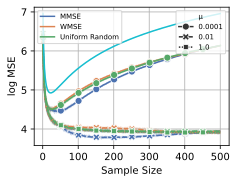
\includegraphics[width=\columnwidth]{figures/proj1/plots/GLR_MSE/ER_0pt8_500_bandwidth_50_SNRdbs_-10.0_samps_500_mus_0.0001_0.01_1_full_band.png}}
    \caption{Full-band noise, SNR = $10^{-1}$}
    \label{GLR_MSE_subfiga}
    \end{subfigure}\hfill
    \begin{subfigure}{0.3\columnwidth}
    \resizebox{\width}{0.62\columnwidth}{
    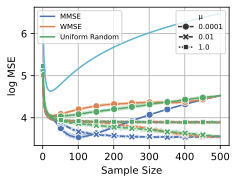
\includegraphics[width=\columnwidth]{figures/proj1/plots/GLR_MSE/ER_0pt8_500_bandwidth_50_SNRdbs_-3.01_samps_500_mus_0.0001_0.01_1_full_band.png}}
    \caption{Full-band noise, SNR = $\frac{1}{2}$}%
    \label{GLR_MSE_subfigb}%
    \end{subfigure}\hfill%
    \begin{subfigure}{0.3\columnwidth}
    \resizebox{\width}{0.62\columnwidth}{
    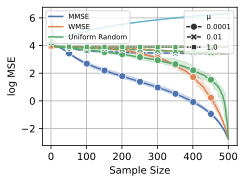
\includegraphics[width=\columnwidth]{figures/proj1/plots/GLR_MSE/ER_0pt8_500_bandwidth_50_SNRdbs_100.0_samps_500_mus_0.0001_0.01_1_full_band.png}}
    \caption{Full-band noise, SNR = $10^{10}$}%
    \label{GLR_MSE_subfigc}%
    \end{subfigure}%
    \caption{Average MSE under GLR on ER Graphs (\#vertices=500, bandwidth = 50), line without markers is an upper bound}
\label{GLR_ER_MSE_fig}
%\label{bandlimited_GLR_ER_MSE_fig}
\end{figure*}

%%% REAL DATASET experiments

\begin{figure}
    \centering
    \begin{subfigure}{0.3\columnwidth}
    %\resizebox{\width}{0.75\columnwidth}
    \resizebox{\width}{0.62\columnwidth}
    {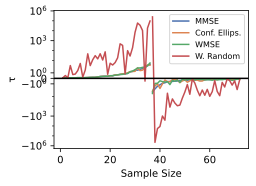
\includegraphics[width=\columnwidth]{figures/proj1/plots/LS_threshold_real/fmri_subsample_500_367_bandwidth_36_thresholds_LS.png}}
    \caption{FMRI} 
    \label{snr_FMRI}
    \end{subfigure}
    \begin{subfigure}{0.3\columnwidth}
    \resizebox{\width}{0.62\columnwidth}{
    \includegraphics[width=\columnwidth]{figures/proj1/plots/LS_threshold_real/weather_45_bandwidth_8_thresholds_LS.png}}
    \caption{Weather}%
    \label{snr_Weather}%
    \end{subfigure}
    \caption{$\tau(\set{S},v)$ for real world datasets under LS and full-band noise}
\label{LS_SNR_Threshold_plots_all_real}
\end{figure}

\begin{figure}%
    \centering
    \begin{subfigure}{0.3\columnwidth}
    \resizebox{\width}{0.62\columnwidth}{
    \includegraphics[width=\columnwidth]{figures/proj1/plots/GLR_threshold_real/fmri_subsample_500_GLR_threshold_fb.png}}
    \caption{FMRI}
    \label{tau_GLR_fmri}
    \end{subfigure}
    \begin{subfigure}{0.3\columnwidth}
    \resizebox{\width}{0.62\columnwidth}{
    \includegraphics[width=\columnwidth]{figures/proj1/plots/GLR_threshold_real/weather_GLR_threshold_fb.png}}
    \caption{Weather}%
    \label{tau_GLR_weather}%
    \end{subfigure}
    \caption{$\tau_{GLR}$ for real world datasets}
\label{GLR_Threshold_plots_real}
\end{figure}


\begin{figure*}%
    \centering
    \begin{subfigure}{0.3\columnwidth}
    \resizebox{\width}{0.62\columnwidth}{
    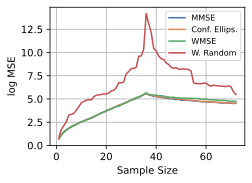
\includegraphics[width=\columnwidth]{figures/proj1/plots/LS_MSE_real/fmri_subsample_500_367_bandwidth_36_SNRdbs_-10.0_samps_72_fb_blsig_MSE_LS.png}}
    \caption{FMRI, SNR = $10^{-1}$}
    \label{fmri_MSE_subfiga}
    \end{subfigure}\hfill
    \begin{subfigure}{0.3\columnwidth}
    \resizebox{\width}{0.62\columnwidth}{
    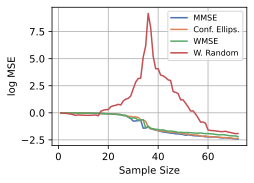
\includegraphics[width=\columnwidth]{figures/proj1/plots/LS_MSE_real/fmri_subsample_500_367_bandwidth_36_SNRdbs_20.0_samps_72_fb_blsig_MSE_LS.png}}
    \caption{FMRI, SNR = $10^{2}$}%
    \label{fmri_MSE_subfigb}%
    \end{subfigure}\hfill%
    \begin{subfigure}{0.3\columnwidth}
    \resizebox{\width}{0.62\columnwidth}{
    \includegraphics[width=\columnwidth]{figures/proj1/plots/LS_MSE_real/fmri_subsample_500_367_bandwidth_36_SNRdbs_100.0_samps_72_fb_blsig_MSE_LS.png}}
    \caption{FMRI, SNR = $10^{10}$}%
    \label{fmri_MSE_subfigc}%
    \end{subfigure}%
    \hfill
    \begin{subfigure}{0.3\columnwidth}
    \resizebox{\width}{0.62\columnwidth}{
    \includegraphics[width=\columnwidth]{figures/proj1/plots/LS_MSE_real/weather_45_bandwidth_8_SNRdbs_-10.0_samps_16_fb_blsig_MSE_LS.png}}
    \caption{Weather, SNR = $10^{-1}$}
    \label{weather_MSE_subfiga}
    \end{subfigure}\hfill
    \begin{subfigure}{0.3\columnwidth}
    \resizebox{\width}{0.62\columnwidth}{
    \includegraphics[width=\columnwidth]{figures/proj1/plots/LS_MSE_real/weather_45_bandwidth_8_SNRdbs_20.0_samps_16_fb_blsig_MSE_LS.png}}
    \caption{Weather, SNR = $1$}%
    \label{weather_MSE_subfigb}%
    \end{subfigure}\hfill%
    \begin{subfigure}{0.3\columnwidth}
    \resizebox{\width}{0.62\columnwidth}{
    \includegraphics[width=\columnwidth]{figures/proj1/plots/LS_MSE_real/weather_45_bandwidth_8_SNRdbs_100.0_samps_16_fb_blsig_MSE_LS.png}}
    \caption{Weather, SNR = $10^{10}$}%
    \label{weather_MSE_subfigc}%
    \end{subfigure}%
    \caption{Average MSE under LS on real world datasets and full-band noise }
\label{LS_real_MSE_fig}
\end{figure*}

\begin{figure*}%
    \centering
    \begin{subfigure}{0.3\columnwidth}
    \resizebox{\width}{0.62\columnwidth}{
    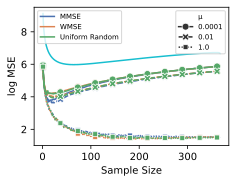
\includegraphics[width=\columnwidth]{figures/proj1/plots/GLR_MSE_real/fmri_subsample_500_367_bandwidth_36_SNRdbs_-10.0_samps_367_mus_0.0001_0.01_1_full_band_MSE_GLR.png}}
    \caption{FMRI, SNR = $10^{-1}$}
    \label{fmri_GLR_MSE_subfiga}
    \end{subfigure}\hfill
    \begin{subfigure}{0.3\columnwidth}
    \resizebox{\width}{0.62\columnwidth}{
    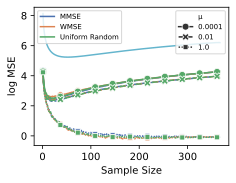
\includegraphics[width=\columnwidth]{figures/proj1/plots/GLR_MSE_real/fmri_subsample_500_367_bandwidth_36_SNRdbs_-3.010299956639812_samps_367_mus_0.0001_0.01_1_full_band_MSE_GLR.png}}
    \caption{FMRI, SNR = $\frac{1}{2}$}%
    \label{fmri_GLR_MSE_subfigb}%
    \end{subfigure}\hfill%
    \begin{subfigure}{0.3\columnwidth}
    \resizebox{\width}{0.62\columnwidth}{
    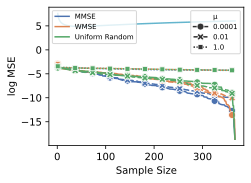
\includegraphics[width=\columnwidth]{figures/proj1/plots/GLR_MSE_real/fmri_subsample_500_367_bandwidth_36_SNRdbs_100.0_samps_367_mus_0.0001_0.01_1_full_band_MSE_GLR.png}}
    \caption{FMRI, SNR = $10^{10}$}%
    \label{fmri_GLR_MSE_subfigc}%
    \end{subfigure}%
    \hfill
    \begin{subfigure}{0.3\columnwidth}
    \resizebox{\width}{0.62\columnwidth}{
    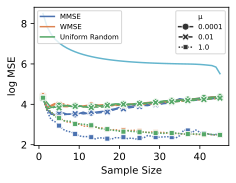
\includegraphics[width=\columnwidth]{figures/proj1/plots/GLR_MSE_real/weather_45_bandwidth_8_SNRdbs_-10.0_samps_45_mus_0.0001_0.01_1_full_band_MSE_GLR.png}}
    \caption{Weather, SNR = $10^{-2}$}
    \label{weather_GLR_MSE_subfiga}
    \end{subfigure}\hfill
    \begin{subfigure}{0.3\columnwidth}
    \resizebox{\width}{0.62\columnwidth}{
    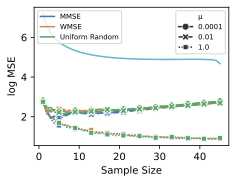
\includegraphics[width=\columnwidth]{figures/proj1/plots/GLR_MSE_real/weather_45_bandwidth_8_SNRdbs_-3.010299956639812_samps_45_mus_0.0001_0.01_1_full_band_MSE_GLR.png}}
    \caption{Weather, SNR = $\frac{1}{2}$}%
    \label{weather_GLR_MSE_subfigb}%
    \end{subfigure}\hfill%
    \begin{subfigure}{0.3\columnwidth}
    \resizebox{\width}{0.62\columnwidth}{
    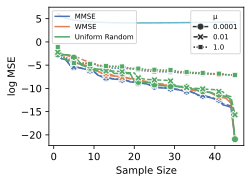
\includegraphics[width=\columnwidth]{figures/proj1/plots/GLR_MSE_real/weather_45_bandwidth_8_SNRdbs_100.0_samps_45_mus_0.0001_0.01_1_full_band_MSE_GLR.png}}
    \caption{Weather, SNR = $10^{10}$}%
    \label{weather_GLR_MSE_subfigc}%
    \end{subfigure}%
    \caption{Average MSE under GLR on real world datasets, line without markers is an upper bound}
\label{GLR_real_MSE_fig}
%\label{bandlimited_GLR_ER_MSE_fig}
\end{figure*}
\fi

Our theoretical results show how the relationship between sample size and MSE changes with the level of noise, focusing on how reducing sample size will reduce MSE if the SNR is below a threshold. In this section, we demonstrate  the applicability and validity of these results via empirical experiments. 

%Note that we always consider SNR in ratio form --- as $10^{x}$ rather than $\frac{x}{10} dB$ --- which is always positive. For the SNR to be below a given threshold (and so for us to show reducing sample size will decrease MSE) the threshold must be positive.

We first demonstrate the applicability of our results with plots of the thresholds $\tau(\set{S},v)$, $\tau_{GLR}$ and $\tau_{GLR\_bl}$ against sample size (Figs. \ref{LS_SNR_Threshold_plots_all} and \ref{GLR_Threshold_plots}). These plots show concrete SNR values for the thresholds, giving a practical understanding of how high noise levels need to be for reducing sample size to reduce MSE for different random graph models and parameters. Additionally, we empirically tabulate the probabilities that graphs from each model  satisfy the conditions of our theorems (Table \ref{tbl:empirical_probabilities_conditions}), allowing the reader to evaluate the impact of our theorems across different applications. We then demonstrate the validity of our results by plotting $\textrm{MSE}_{\set{S}}$ against sample size (Figs. \ref{LS_ER_MSE_fig} and  \ref{GLR_ER_MSE_fig}) at SNRs below, near and above the derived thresholds, showing that the behaviour of $\textrm{MSE}_{\set{S}}$ follows our theoretical results. \bs{We finally present similar results on real-world datasets, validating the applicability of our results to real world datasets.}

\subsection{Experimental Setup}
We now present the setup of the experiments. All results are presented with 90\% confidence intervals and all experiments use the combinatorial Laplacian $\matr{L}$ and its eigenbasis.
\subsubsection{\bs{Synthetic} Graph Generation}
We consider each of the following unweighted random graph models:
\begin{itemize}
    \item Erdős–Rényi (ER) with edge probability $p=0.8$ (experiments with other values of $p$ show similar results)
    \item Barabási-Albert (BA) with a preferential attachment to 3 vertices at each step of its construction
    \item Stochastic Blockmodel (SBM) with intra- and inter-cluster edge probabilities of $0.7 \text{ and }0.1$ respectively
    %\item Ring (Ring).
\end{itemize}
We consider 10 instantiations of each model for plots, and 1000 instantiations of each model to assess the probability the graph invariant conditions in our Theorems are met.

We present threshold plots for graphs with 500, 1000, 2000 and 3000 vertices. We only present MSE plots for graphs with 500 vertices  {\color{black}  (like \cite[Fig 8]{bai2020fast})} as they are intended as an accompaniment to our threshold plots and theorems to demonstrate their validity, and a single graph size suffices. 

\subsubsection{\xd{Synthetic} Signal Generation}
We set the bandwidth  $k = \lfloor \frac{N}{10} \rfloor$, as per \cite{bai2020fast}.  We consider the following SNRs:

\begin{itemize}
    \item \makebox[4.1\labelwidth][l]{Full-band noise:} $10^{-1},\ 0.5,\ 10^{10}$ (i.e. $-10\,\mathrm{dB},\ -3\,\mathrm{dB},\ 100\,\mathrm{dB}$)
    \item \makebox[4.1\labelwidth][l]{Bandlimited noise:} $10^{-2},\ 0.5,\ 10^{10}$ (i.e. $-20\,\mathrm{dB},\ -3\,\mathrm{dB},\ 100\,\mathrm{dB}$)
\end{itemize}




These SNRs are chosen to demonstrate that there are three regimes for MSE with distinctive properties---the high noise regime, the transitionary regime and the approximately noiseless regime---and that $\tau$ captures when the regimes change. Suitable values of SNRs to demonstrate this vary between reconstruction methods and noise types, hence our choices.
%Note that we always consider SNR in ratio form---as $10^{x}$ rather than $\frac{x}{10} dB$---which is always positive. For the SNR to be below a given threshold (and so for us to show reducing sample size will decrease MSE) the threshold must be positive.

To test the MSE in reconstructing signals from samples \bs{on random graph models}, we generate 200 signals by sampling $\vect{y} = \vect{x}_{raw} + \sigma \cdot \epsilon_{raw}$ where:
\begin{enumerate}
    \item $\vect{x}_{raw} \sim \mathcal{N}(\vect{0}, \matr{\Pi}_{bl(\set{K})})$ 
    \item[2a)] If full-band noise, $\vect{\epsilon}_{raw} \sim \mathcal{N}(\vect{0}, \matr{I}_{N})$, $\sigma = \sqrt{\frac{k}{{N \cdot\text{SNR}}}}$
    \item[2b)]  If bandlimited noise, $\vect{\epsilon}_{raw} \sim \mathcal{N}(\vect{0}, \projbl )$, $\sigma = \frac{1}{\sqrt{\text{SNR}}}$ 
    %\item Normalise $\vect{x}_{raw}$ and $\vect{\epsilon}_{raw}$ to have norm 1
    %\item Normalise: $\vect{x} = \frac{\vect{x}_{raw}}{||\vect{x}_{raw}||_{2}}$ and $\vect{\epsilon} = \frac{\vect{\epsilon}_{raw}}{ ||\vect{\epsilon}_{raw}||_{2}}$
    %\item[3)] Return $\vect{y} = \vect{x} + \frac{\vect{\epsilon}}{\sqrt{\text{SNR}}}$
    %\item[3)] Return $\vect{y} = \vect{x} + \sigma \cdot \epsilon$
\end{enumerate}
%For the cases of bandlimited noise, in step (1) we generate $\vect{\epsilon}_{raw} \sim \mathcal{N}(\vect{0}, \projbl )$ instead.

\subsubsection{Real World Datasets}
\bs{
We also consider two real world datasets as in \cite{zhi2023gaussian}. The first is an FMRI dataset, where the original graph consists of 4465 nodes corresponding to voxels of the cerebellum, with 292 Blood-Oxygen-Level-Dependent (BOLD) signals derived from FMRI. We sample a connected subgraph of 367 nodes via Neighbourhood Sampling \cite{hamilton2017inductive}. The second is a Weather dataset, where a $10$-nearest neighbours graph of 45 cities in Sweden is constructed, with 95 signals derived from the temperature. See \cite{venkitaraman2020gaussian, behjat2016signal, zhi2023gaussian} for details on graph construction and signal generation in both cases. 
We generate $\vect{x}$ by $k$-bandlimiting the original signals, where For FMRI we set $k=36$ and for Weather dataset we set $k=8$. We otherwise follow the above methodology in Synthetic Signal Generation for generating signals with full-band noise.
}


\subsubsection{Sample-Set Selection}
%The literature provides several approximations to make vertex sample-set selection efficient; for example, approximating the projection matrix $\projbl$ \cite{wang2018optimal} (subsets of which are used to compute optimality criteria) with a polynomial in $\matr{L}$, and approximating optimality criteria for easier computation \cite{bai2020fast}. 

We generate sample sets greedily using exact analytic forms and by exactly computing $\matr{\Pi}_{bl(\set{K})}$.
\begin{itemize}
    \item[GLR:] We exactly compute the MMSE criterion, which is a function of SNR and noise type, and the WMSE criterion {\color{black}\cite{EOptimalChen}}, which is not. We also consider uniform random sampling.
\end{itemize}
Note that sampling schemes in the literature tend to differ from ours mainly in that they approximate our setup for computational efficiency reasons; e.g. approximating the projection matrix $\projbl$ with a polynomial in $\matr{L}$ \cite{wang2018optimal}, and approximating optimality criteria \cite{bai2020fast}. As these differences are for efficiency reasons, we do not expect them to matter in our experiments.

\subsubsection{Parameters of Reconstruction Methods} We consider GLR with $\mu \in \{10^{-4}, 10^{-2}, 1 \}$.

\subsection{Experimental Results --- Synthetic Graphs}

%GLR_threshold_plots

\begin{figure*}[h]%
    \centering
    \begin{subfigure}{0.3\columnwidth}
    \resizebox{\width}{0.62\columnwidth}{
    \includegraphics[width=\columnwidth]{figures/proj1/plots/GLR_threshold/ER_fb.png}}
    \caption{Erdős–Rényi ($\tau_{GLR}$)}
    \label{tau_GLR_er}
    \end{subfigure}
    \hfill
    \begin{subfigure}{0.3\columnwidth}
    \resizebox{\width}{0.62\columnwidth}{
    \includegraphics[width=\columnwidth]{figures/proj1/plots/GLR_threshold/BA_fb.png}}
    \caption{Barabási-Albert($\tau_{GLR}$)}%
    \label{tau_GLR_BA}%
    \end{subfigure}
    \hfill%
    \begin{subfigure}{0.3\columnwidth}
    \resizebox{\width}{0.62\columnwidth}{
    \includegraphics[width=\columnwidth]{figures/proj1/plots/GLR_threshold/SBM_fb.png}}
    \caption{SBM ($\tau_{GLR}$)}%
    \label{tau_GLR_SBM}%
    \end{subfigure}%
    \hfill
    \caption{$\tau_{GLR}$  for different random graph models (\#vertices = colour, bandwidth = $\frac{\text{\# vertices}}{10}$)}
\label{GLR_Threshold_plots}
\end{figure*}


\begin{figure*}[h]%
    \centering
    \begin{subfigure}{0.3\columnwidth}
    \resizebox{\width}{0.62\columnwidth}{
    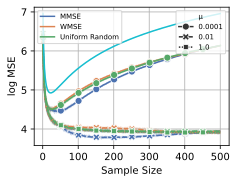
\includegraphics[width=\columnwidth]{figures/proj1/plots/GLR_MSE/ER_0pt8_500_bandwidth_50_SNRdbs_-10.0_samps_500_mus_0.0001_0.01_1_full_band.png}}
    \caption{Full-band noise, SNR = $10^{-1}$}
    \label{GLR_MSE_subfiga}
    \end{subfigure}\hfill
    \begin{subfigure}{0.3\columnwidth}
    \resizebox{\width}{0.62\columnwidth}{
    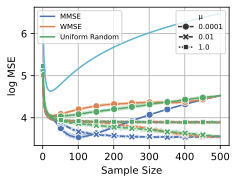
\includegraphics[width=\columnwidth]{figures/proj1/plots/GLR_MSE/ER_0pt8_500_bandwidth_50_SNRdbs_-3.01_samps_500_mus_0.0001_0.01_1_full_band.png}}
    \caption{Full-band noise, SNR = $\frac{1}{2}$}%
    \label{GLR_MSE_subfigb}%
    \end{subfigure}\hfill%
    \begin{subfigure}{0.3\columnwidth}
    \resizebox{\width}{0.62\columnwidth}{
    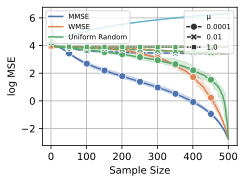
\includegraphics[width=\columnwidth]{figures/proj1/plots/GLR_MSE/ER_0pt8_500_bandwidth_50_SNRdbs_100.0_samps_500_mus_0.0001_0.01_1_full_band.png}}
    \caption{Full-band noise, SNR = $10^{10}$}%
    \label{GLR_MSE_subfigc}%
    \end{subfigure}%
    \caption{Average MSE under GLR on ER Graphs (\#vertices=500, bandwidth = 50), line without markers is an upper bound}
\label{GLR_ER_MSE_fig}
%\label{bandlimited_GLR_ER_MSE_fig}
\end{figure*}


For full-band noise, we present threshold plots for all graphs and MSE plots for ER graphs in the main body of the paper. MSE plots for BA and SBM graphs are presented in Appendix \ref{plot_appendix}. For bandlimited noise, we present threshold plots, MSE plots and discussion of how the experimental and theoretical results correspond in Appendix \ref{app:Experiments_Bandlimited}.
{\color{black} We also present Table \ref{tbl:theory_experiment_correspondence} showing how our plots correspond to our theoretical results, which also corresponds to the summary of theoretical results in Table \ref{tbl:general_theory}.}

\iffalse
\begin{table}[h]
{\color{black}
\caption{Correspondence of Theory and Empirical Results}
\centering
\begin{tabularx}{(\textwidth)}{|X|p{2.6cm}|p{2.5cm}|p{2.6cm}|p{2.6cm}|}%{|@{\hspace{0.1cm}}p{2.6cm}|p{2.6cm}|p{2.6cm}|p{2.6cm}|X|}
\hline
\multirow{2}{*}{} & \multicolumn{2}{c|}{\textbf{LS}} & \multicolumn{2}{c|}{\textbf{GLR}} \\
\cline{2-5}
 & Full-band & Bandlimited & Full-band & Bandlimited \\
\hline
\textbf{Character- isation} & 
\makecell{Corr \ref{main_ls} \\
(Figs. \ref{snr_ER}-\ref{snr_SBM}\\
\& \ref{MSE_subfiga}-\ref{MSE_subfigc})} & 
\makecell{Corr \ref{corr:LS_bandlimited_noise_big_variance} \\ (Figs. \ref{bandlimited_MSE_subfiga}-\\ \ref{bandlimited_MSE_subfigc})} & 
\multicolumn{2}{c|}{\makecell{Corr \ref{corr:main_GLR_iff} \\ (Figs. \ref{GLR_MSE_subfiga}-\ref{GLR_MSE_subfigc})}
} \\
\hline
\textbf{Existence} & 
\makecell{Thm \ref{thm:noiseless_optimality_means_noise_sensitivity} \\ (Figs. \ref{snr_ER}-\ref{snr_SBM}\\
\& \ref{MSE_subfiga}-\ref{MSE_subfigc})} & 
\makecell{Corr \ref{corr:LS_bandlimited_noise_sample_only_k} \\ (Figs. \ref{bandlimited_MSE_subfiga}- \\ \ref{bandlimited_MSE_subfigc})} & 
\makecell{Thm \ref{thm:main_GLR_exist} \\
 (Figs. \ref{tau_GLR_er}-\ref{tau_GLR_SBM} \\ \& \ref{GLR_MSE_subfiga}-\ref{GLR_MSE_subfigc}\\
 \& Table \ref{tbl:empirical_probabilities_conditions})
} & 
\makecell{Thm \ref{thm:main_GLR_bl} \\
(Figs. \ref{tau_GLR_bl_er}-\ref{tau_GLR_bl_SBM} \\ \& \ref{bandlimited_GLR_MSE_subfiga}-\ref{bandlimited_GLR_MSE_subfigc} \\
\& Table \ref{tbl:empirical_probabilities_conditions_bl})
} \\
\hline
\textbf{Asymptotics} & 
\makecell{Rmk \ref{rmk:LS_big_N} \\ (Figs. \ref{snr_ER_1000}-\ref{snr_ER_3000})} & 
\makecell{\\ Rmk \ref{rmk:LS_big_N_bl}} & 
\makecell{Propn \ref{propn:GLR_big_N} \\ (Figs. \ref{tau_GLR_er}-\ref{tau_GLR_SBM})} & 
\makecell{Propn \ref{propn:GLR_big_N_bl} \\ (Figs. \ref{tau_GLR_bl_er}-\ref{tau_GLR_bl_SBM})} \\
\hline
\end{tabularx}
\label{tbl:theory_experiment_correspondence}
}
\end{table}
\fi

% Table 2: GLR columns only
\begin{table}[h]
\caption{Correspondence of Theory and Empirical Results - GLR}
\centering
\begin{tabularx}{(\textwidth)}{l >{\centering\arraybackslash}X >{\centering\arraybackslash}X}
\toprule
& \multicolumn{2}{c}{\textbf{GLR}} \\
\cmidrule(lr){2-3}
 & Full-band Noise & Bandlimited Noise \\
\midrule
\textbf{Characterisation} & 
{\makecell{Corr \ref{corr:main_GLR_iff} \\ (Figs. \ref{GLR_MSE_subfiga}-\ref{GLR_MSE_subfigc})}
} & {\makecell{Corr \ref{corr:main_GLR_iff} \\ (Figs. \ref{GLR_MSE_subfiga}-\ref{GLR_MSE_subfigc})}
} \\
\midrule
\textbf{Existence} & 
\makecell[c]{Thm \ref{thm:main_GLR_exist} \\
 (Figs. \ref{tau_GLR_er}-\ref{tau_GLR_SBM} \\ \& \ref{GLR_MSE_subfiga}-\ref{GLR_MSE_subfigc}\\
 \& Table \ref{tbl:empirical_probabilities_conditions})
} & 
\makecell[c]{Thm \ref{thm:main_GLR_bl} \\
(Figs. \ref{tau_GLR_bl_er}-\ref{tau_GLR_bl_SBM} \\ \& \ref{bandlimited_GLR_MSE_subfiga}-\ref{bandlimited_GLR_MSE_subfigc} \\
\& Table \ref{tbl:empirical_probabilities_conditions_bl})
} \\
\midrule
\textbf{Asymptotics} & 
\makecell[c]{Propn \ref{propn:GLR_big_N} \\ (Figs. \ref{tau_GLR_er}-\ref{tau_GLR_SBM})} & 
\makecell[c]{Propn \ref{propn:GLR_big_N_bl} \\ (Figs. \ref{tau_GLR_bl_er}-\ref{tau_GLR_bl_SBM})} \\
\bottomrule
\end{tabularx}
\label{tbl:theory_experiment_correspondence_GLR}
\end{table}


%\subsubsection{\texorpdfstring{$\tau$ and $\tau_{GLR}$ plots}{\texttau and \texttau\_GLR plots}}
\subsubsection{$\tau_{GLR}$ plots (GLR)}
%\emph{[GLR]:}  
In Figs. \ref{tau_GLR_er}-\ref{tau_GLR_SBM}, we plot $\tau_{GLR}$, where if $\textrm{SNR} < \tau_{GLR}$, then there is a sample size $m_{opt} < N$ where \emph{any} sample set of size $m_{opt}$ is better than $\set{N}$. Unlike with LS, our theorems are only sufficient so $\text{SNR} > \tau_{GLR}$ is uninformative. %We interpret the subplots of Fig. \ref{GLR_Threshold_plots}:
%%Figs. \ref{GLR_Threshold_plots} and \ref{bandlimited_GLR_Threshold_plots} plot $\tau_{GLR}$ and $\tau_{GLR_bl}$. 
% \begin{itemize}
    % \item[(a)] 
    For ER graphs, we see that $\tau_{GLR}$ is decreasing in $\mu$, and that $\tau_{GLR} > 0$ for sufficiently small $\mu$ for all graph sizes. The maximum value in this case for $\tau_{GLR}$ ranges between 0.4 ($-4dB$) and 0.7 ($-1.5dB$). %and the confidence intervals are very tight.
    We see a similar pattern to ER graphs for BA graphs, the main differences being that $\tau_{GLR} > 0$ for larger values of $\mu$ and that the maxmimum of $\tau_{GLR}$ is  approximately {\color{black}0.2 ($-7dB$)}.
    $\tau_{GLR}$ for SBM graphs behaves very similarly to ER graphs in our experiments.
% \end{itemize}
%We can think of $\tau_{GLR}$ as a lower bound for upper bounds for SNR --- if $\textrm{SNR} < \tau_{GLR}$ we can definitely reduce sample size to reduce MSE, but we can say nothing in the case $\textrm{SNR} \geq \tau_{GLR}$.
Note that the confidence intervals for ER and SBM graphs are so tight as to not be clearly seen in Fig. \ref{GLR_Threshold_plots}, while being much wider for BA graphs. As  graph properties, when we sample from a random graph model, $r$ is a random variables. We observe wider confidence intervals {\color{black}when $\mathcal{G}$ is sampled from the BA graph model as $\text{Var}_{\mathcal{G}}(r)$ is much higher than when we sample from the ER or SBM graph models.}
%This is because the variance of $r$ and $\rho$ across different instances of the graph models are much higher for BA graphs than for ER and SBM graphs. 

As $\tau_{GLR} > 0$, Figs. \ref{tau_GLR_er}-\ref{tau_GLR_SBM} show we can reduce sample size to reduce MSE for all examined graph models. We see $\tau_{GLR}$ is only positive for small enough $\mu$, motivating $\mu_{ub}$ in Theorem \ref{thm:main_GLR_exist}. The value of $\mu$ below which $\tau_{GLR} > 0$ is at least $\mu_{ub}$.

Finally, Proposition \ref{propn:GLR_big_N} proves that $\tau_{GLR} \not\to 0$ as $N \to \infty$ for $\mu = \frac{c}{\lambda_{2}}$,  or $\frac{c}{\lambda_{N}}$, or $\frac{c}{\sqrt{\lambda_{2}\lambda_{N}} }$ on ER graphs, i.e. for decreasing $\mu$ as $N$ increases. We note that Figs. \ref{tau_GLR_er}-\ref{tau_GLR_SBM}  provide empirical evidence that this might hold for all graph models tested.


\subsubsection{MSE plots (GLR)}
As with LS, the MSE plots demonstrate the validity of our theoretical results linking MSE and sample size.
%\emph{[GLR]:}
Figs. \ref{GLR_MSE_subfiga}-\ref{GLR_MSE_subfigc} show how MSE changes with sample size for different values of $\mu$ under full-band noise, along with an upper bound (light blue) which is not dependent on $\mu$. This bound is approximately U-shaped in all cases.
% \begin{itemize}
    % \item[(a)] 
    For $\text{SNR} = 10^{-1}$, we see for $\mu=10^{-4}$, under all sampling schemes, MSE is minimised at a sample size around 16 to 22. For the MMSE sampling scheme with $\mu=0.01$, MSE is minimised at a sample size of approximately 200. In all other cases where $\text{SNR} = 10^{-1}$, MSE is minimised at full observation $(|\set{S}|=500)$.
    For $\text{SNR}=\frac{1}{2}$ and $\mu=10^{-4}$, MSE is minimised at a sample size a bit less than 100. For larger $\mu$, we see MSE is minimised at full observation.
    In the nearly noiseless case, MSE decreases with sample size under all parameter choices. In all cases where the MSE is minimised at a sample size less than $N$, the MSE is approximately U-shaped like our bound {\color{black} and 
 our diagram Fig. \ref{fig:GLR_diagram}}.
% \end{itemize}


Figs. \ref{GLR_MSE_subfiga}-\ref{GLR_MSE_subfigc} illustrate Corollary \ref{corr:main_GLR_iff}, Theorem \ref{thm:main_GLR_exist} and Corollary \ref{corr:unif_ub_xi_1_MSE} in the following ways. First, the MSE upper bound corresponds to Corollary \ref{corr:unif_ub_xi_1_MSE}, and we can see it is greater than any observed MSE at each sample size. The sample size which minimises our upper bound is $m_{opt}$ (Remark \ref{remark:mopt}) and as $r \in (1,1.01]$ in our Erdős–Rényi experiments, $m_{opt} \in [22,23]$, which empirically well approximates the sample size that minimises MSE in our low $\mu$ and low SNR experiments. %However, $\sqrt{N}$ is a good estimate of the true optimal sample size at low $\mu$ and low $\textrm{SNR}$, as can be seen in Fig. \ref{GLR_MSE_subfiga}.
Second, Figs. \ref{GLR_MSE_subfiga}-\ref{GLR_MSE_subfigc} show that MSE can decrease with increasing sample size, and Fig. \ref{GLR_MSE_subfigc} shows that at high SNR full observation is best, illustrating the necessary and sufficient nature of Corollary \ref{corr:main_GLR_iff}.
Finally, Figs. \ref{GLR_MSE_subfiga}-\ref{GLR_MSE_subfigc} illustrate the dependence on SNR and $\mu$ in Theorem \ref{thm:main_GLR_exist}, i.e. at low $\mu$ and SNR the optimal sample size is less than $N$, but at high enough $\mu$ or SNR this no longer holds.  

Figs. \ref{GLR_MSE_subfiga}-\ref{GLR_MSE_subfigc} also demonstrate some limitations of the characterisation in Corollary \ref{corr:unif_ub_xi_1_MSE} and Theorem \ref{thm:main_GLR_exist}. We see from Fig. \ref{GLR_MSE_subfigb} that even though the MSE at $m_{opt}$ is lower than at $N$, our bound never goes below the maximum observed MSE, so is too loose to show this. This is partly because the Theorem and the Corollary bound $\xi_{2}(\set{S})$ only as a function of $|\set{S}|$, ignoring $\mu$ and the composition of $\set{S}$. This limitation corresponds to a gap between $\tau_{GLR}$ and $\tau(\set{N},\set{S}^{c})$, demonstrating $\tau_{GLR}$ is a lower bound for $\tau(\set{N},\set{S}^{c})$ rather than an exact characterisation.


\subsubsection{Checking Conditions}
While our theorems for LS apply to all graphs, Theorem \ref{thm:main_GLR_exist} for GLR relies on conditions around graph invariants. We sample graphs from each random graph model to empirically show the probability the conditions of Theorem \ref{thm:main_GLR_exist} are met at a sample size of $m_{opt}$ for some $\mu > 0$:

\begin{table}[h!]
\caption{Probability theorem conditions are met}
    \begin{center}
        \begin{tabular}{lccc}
        \toprule
        & \textbf{ER} & \textbf{SBM} & \textbf{BA} \\ 
        \midrule
        Theorem \ref{thm:main_GLR_exist} conditions met & 100\% & 100\% & 99.9\% \\ 
        % Theorem \ref{thm:main_GLR_bl} conditions met & 100\% & 100\% & 99.4\% \\
        \bottomrule
        \end{tabular}
    \end{center}
    \label{tbl:empirical_probabilities_conditions}
\end{table}

Proposition \ref{propn:GLR_big_N} shows the conditions in Theorem \ref{thm:main_GLR_exist} hold w.h.p. for ER graphs as $N \to \infty$. However, the proposition does not say whether the conditions hold for a graph of a given size, or other graph models. The results in Table \ref{tbl:empirical_probabilities_conditions} show empirically that the conditions hold under full-band noise (Theorem \ref{thm:main_GLR_exist}) for ER, BA and SBM graphs with $500$ vertices. This outlines the applicability of our theorems.

If the conditions on our Theorems are not met, they provide no information about the shape of the MSE. However, Figs. \ref{bandlimited_GLR_BA_MSE_fig} and  \ref{bandlimited_GLR_SBM_MSE_fig} in Appendix \ref{plot_appendix} show empirically that for BA and SBM graphs under bandlimited noise with $\text{SNR} \in \{10^{-2}, \frac{1}{2}\}$ under GLR with $\mu \in 
\{10^{-2}, 10^{-4}\}$, even if the conditions of Theorem \ref{thm:main_GLR_bl} are not met, reducing sample size from ${N}$ to below ${N}$ reduces MSE under the presented sampling schemes. We leave further investigation of this as future work. %It is future work to sharpen Theorem \ref{thm:main_GLR_bl} to include these cases.

{\color{black}
\subsection{Experimental Results --- Real World Datasets}

%%% REAL DATASET experiments

\begin{figure}%
    \centering
    \begin{subfigure}{0.31\columnwidth}
    \resizebox{\width}{0.62\columnwidth}{
    \includegraphics[width=\columnwidth]{figures/proj1/plots/GLR_threshold_real/fmri_subsample_500_GLR_threshold_fb.png}}
    \caption{FMRI}
    \label{tau_GLR_fmri}
    \end{subfigure}
    \begin{subfigure}{0.31\columnwidth}
    \resizebox{\width}{0.62\columnwidth}{
    \includegraphics[width=\columnwidth]{figures/proj1/plots/GLR_threshold_real/weather_GLR_threshold_fb.png}}
    \caption{Weather}%
    \label{tau_GLR_weather}%
    \end{subfigure}
    \caption{$\tau_{GLR}$ for real world datasets}
\label{GLR_Threshold_plots_real}
\end{figure}


\begin{figure*}%
    \centering
    \begin{subfigure}{0.3\columnwidth}
    \resizebox{\width}{0.62\columnwidth}{
    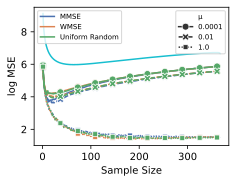
\includegraphics[width=\columnwidth]{figures/proj1/plots/GLR_MSE_real/fmri_subsample_500_367_bandwidth_36_SNRdbs_-10.0_samps_367_mus_0.0001_0.01_1_full_band_MSE_GLR.png}}
    \caption{FMRI, SNR = $10^{-1}$}
    \label{fmri_GLR_MSE_subfiga}
    \end{subfigure}\hfill
    \begin{subfigure}{0.3\columnwidth}
    \resizebox{\width}{0.62\columnwidth}{
    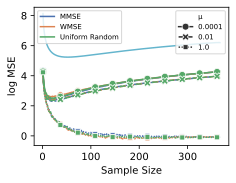
\includegraphics[width=\columnwidth]{figures/proj1/plots/GLR_MSE_real/fmri_subsample_500_367_bandwidth_36_SNRdbs_-3.010299956639812_samps_367_mus_0.0001_0.01_1_full_band_MSE_GLR.png}}
    \caption{FMRI, SNR = $\frac{1}{2}$}%
    \label{fmri_GLR_MSE_subfigb}%
    \end{subfigure}\hfill%
    \begin{subfigure}{0.3\columnwidth}
    \resizebox{\width}{0.62\columnwidth}{
    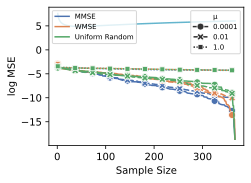
\includegraphics[width=\columnwidth]{figures/proj1/plots/GLR_MSE_real/fmri_subsample_500_367_bandwidth_36_SNRdbs_100.0_samps_367_mus_0.0001_0.01_1_full_band_MSE_GLR.png}}
    \caption{FMRI, SNR = $10^{10}$}%
    \label{fmri_GLR_MSE_subfigc}%
    \end{subfigure}%
    \hfill
    \begin{subfigure}{0.3\columnwidth}
    \resizebox{\width}{0.62\columnwidth}{
    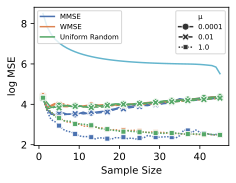
\includegraphics[width=\columnwidth]{figures/proj1/plots/GLR_MSE_real/weather_45_bandwidth_8_SNRdbs_-10.0_samps_45_mus_0.0001_0.01_1_full_band_MSE_GLR.png}}
    \caption{Weather, SNR = $10^{-2}$}
    \label{weather_GLR_MSE_subfiga}
    \end{subfigure}\hfill
    \begin{subfigure}{0.3\columnwidth}
    \resizebox{\width}{0.62\columnwidth}{
    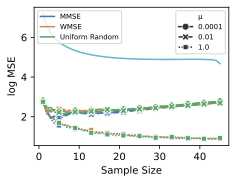
\includegraphics[width=\columnwidth]{figures/proj1/plots/GLR_MSE_real/weather_45_bandwidth_8_SNRdbs_-3.010299956639812_samps_45_mus_0.0001_0.01_1_full_band_MSE_GLR.png}}
    \caption{Weather, SNR = $\frac{1}{2}$}%
    \label{weather_GLR_MSE_subfigb}%
    \end{subfigure}\hfill%
    \begin{subfigure}{0.3\columnwidth}
    \resizebox{\width}{0.62\columnwidth}{
    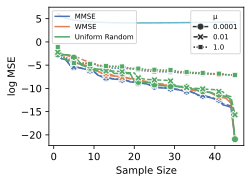
\includegraphics[width=\columnwidth]{figures/proj1/plots/GLR_MSE_real/weather_45_bandwidth_8_SNRdbs_100.0_samps_45_mus_0.0001_0.01_1_full_band_MSE_GLR.png}}
    \caption{Weather, SNR = $10^{10}$}%
    \label{weather_GLR_MSE_subfigc}%
    \end{subfigure}%
    \caption{Average MSE under GLR on real world datasets, line without markers is an upper bound}
\label{GLR_real_MSE_fig}
%\label{bandlimited_GLR_ER_MSE_fig}
\end{figure*}

We first discuss the plots of $\tau_{GLR}$ for real world datasets. In practice, one cannot know for sure what the signal model of a real world signal is; however, computation of $\tau_{GLR}$ is dependent on our choice of theoretical signal model. We have therefore computed $\tau$ under the signal model assumptions given in Section \ref{sec:signal_model}.  
}
%By Proposition \ref{propn:averages_generalise_to_forall}, we know that there is a threshold $\tau > 0$ whenever $\tau$ is positive under our bandlimited signal model. This means that we have proven the sign of $\tau$ in \ref{LS_SNR_Threshold_plots_all_real} is correct, even though our assumption that the covariance of the signal model is $\projbl$ may not hold. We validate the accuracy of the value of our computed $\tau(\set{S},v)$ in our discussion of the MSE plots.

\subsubsection{$\tau$ plots (GLR)}
By Theorem \ref{thm:main_GLR_exist}, $\tau_{GLR}$ being positive means $\tau(\set{N},\set{S}^{C}) >0$ under the bandlimited signal model. As Theorem \ref{thm:main_GLR_exist} functions by showing $\Delta_{2} >0$, by Proposition \ref{propn:averages_generalise_to_forall}, $\tau_{GLR}$ being positive under one signal model means $\tau(\set{N},\set{S}^{C})$ is positive under any signal model. We use this to interpret Fig. \ref{GLR_Threshold_plots_real}.
We can see from Fig. \ref{tau_GLR_fmri} that if $\mu<0.01$ then at some noise level, any set of size $m_{opt}$ is better than $\set{N}$. Fig. \ref{tau_GLR_weather} which shows $\tau_{GLR} < 0$ for all $\mu$ is completely uninformative -- $\tau_{GLR}$ is a lower bound for $\tau(\set{N},\set{S}^{C})$, and a negative lower bound cannot tell us whether the bounded quantity is or isn't positive. We validate this in the MSE section.

\subsubsection{MSE plots (GLR)}
All four figures in Fig. \ref{GLR_real_MSE_fig} corresponding to $\text{SNR} \leq \frac{1}{2}$ and $\mu < 1$ show the minimum MSE at sample size of significantly less than $N$, which validates Theorem \ref{thm:main_GLR_exist} combined with Proposition \ref{propn:averages_generalise_to_forall}. This is expected for the FMRI graph for $\mu<0.01$, as $\tau_{GLR} > 0$ and we had proof that decreasing sample size from $N$ would decrease MSE. However, it is the case for the Weather graph, even though our computation of $\tau_{GLR}$ was negative; this is not unexpected as Theorem \ref{thm:main_GLR_exist} is sufficient but not necessary.

